% Options for packages loaded elsewhere
\PassOptionsToPackage{unicode}{hyperref}
\PassOptionsToPackage{hyphens}{url}
%
\documentclass[
]{article}
\usepackage{amsmath,amssymb}
\usepackage{lmodern}
\usepackage{iftex}
\ifPDFTeX
  \usepackage[T1]{fontenc}
  \usepackage[utf8]{inputenc}
  \usepackage{textcomp} % provide euro and other symbols
\else % if luatex or xetex
  \usepackage{unicode-math}
  \defaultfontfeatures{Scale=MatchLowercase}
  \defaultfontfeatures[\rmfamily]{Ligatures=TeX,Scale=1}
\fi
% Use upquote if available, for straight quotes in verbatim environments
\IfFileExists{upquote.sty}{\usepackage{upquote}}{}
\IfFileExists{microtype.sty}{% use microtype if available
  \usepackage[]{microtype}
  \UseMicrotypeSet[protrusion]{basicmath} % disable protrusion for tt fonts
}{}
\makeatletter
\@ifundefined{KOMAClassName}{% if non-KOMA class
  \IfFileExists{parskip.sty}{%
    \usepackage{parskip}
  }{% else
    \setlength{\parindent}{0pt}
    \setlength{\parskip}{6pt plus 2pt minus 1pt}}
}{% if KOMA class
  \KOMAoptions{parskip=half}}
\makeatother
\usepackage{xcolor}
\IfFileExists{xurl.sty}{\usepackage{xurl}}{} % add URL line breaks if available
\IfFileExists{bookmark.sty}{\usepackage{bookmark}}{\usepackage{hyperref}}
\hypersetup{
  pdftitle={Data Analysis Coursebook},
  pdfauthor={Marcell Granat \& Zoltan Madari},
  hidelinks,
  pdfcreator={LaTeX via pandoc}}
\urlstyle{same} % disable monospaced font for URLs
\usepackage[margin=1in]{geometry}
\usepackage{color}
\usepackage{fancyvrb}
\newcommand{\VerbBar}{|}
\newcommand{\VERB}{\Verb[commandchars=\\\{\}]}
\DefineVerbatimEnvironment{Highlighting}{Verbatim}{commandchars=\\\{\}}
% Add ',fontsize=\small' for more characters per line
\usepackage{framed}
\definecolor{shadecolor}{RGB}{248,248,248}
\newenvironment{Shaded}{\begin{snugshade}}{\end{snugshade}}
\newcommand{\AlertTok}[1]{\textcolor[rgb]{0.94,0.16,0.16}{#1}}
\newcommand{\AnnotationTok}[1]{\textcolor[rgb]{0.56,0.35,0.01}{\textbf{\textit{#1}}}}
\newcommand{\AttributeTok}[1]{\textcolor[rgb]{0.77,0.63,0.00}{#1}}
\newcommand{\BaseNTok}[1]{\textcolor[rgb]{0.00,0.00,0.81}{#1}}
\newcommand{\BuiltInTok}[1]{#1}
\newcommand{\CharTok}[1]{\textcolor[rgb]{0.31,0.60,0.02}{#1}}
\newcommand{\CommentTok}[1]{\textcolor[rgb]{0.56,0.35,0.01}{\textit{#1}}}
\newcommand{\CommentVarTok}[1]{\textcolor[rgb]{0.56,0.35,0.01}{\textbf{\textit{#1}}}}
\newcommand{\ConstantTok}[1]{\textcolor[rgb]{0.00,0.00,0.00}{#1}}
\newcommand{\ControlFlowTok}[1]{\textcolor[rgb]{0.13,0.29,0.53}{\textbf{#1}}}
\newcommand{\DataTypeTok}[1]{\textcolor[rgb]{0.13,0.29,0.53}{#1}}
\newcommand{\DecValTok}[1]{\textcolor[rgb]{0.00,0.00,0.81}{#1}}
\newcommand{\DocumentationTok}[1]{\textcolor[rgb]{0.56,0.35,0.01}{\textbf{\textit{#1}}}}
\newcommand{\ErrorTok}[1]{\textcolor[rgb]{0.64,0.00,0.00}{\textbf{#1}}}
\newcommand{\ExtensionTok}[1]{#1}
\newcommand{\FloatTok}[1]{\textcolor[rgb]{0.00,0.00,0.81}{#1}}
\newcommand{\FunctionTok}[1]{\textcolor[rgb]{0.00,0.00,0.00}{#1}}
\newcommand{\ImportTok}[1]{#1}
\newcommand{\InformationTok}[1]{\textcolor[rgb]{0.56,0.35,0.01}{\textbf{\textit{#1}}}}
\newcommand{\KeywordTok}[1]{\textcolor[rgb]{0.13,0.29,0.53}{\textbf{#1}}}
\newcommand{\NormalTok}[1]{#1}
\newcommand{\OperatorTok}[1]{\textcolor[rgb]{0.81,0.36,0.00}{\textbf{#1}}}
\newcommand{\OtherTok}[1]{\textcolor[rgb]{0.56,0.35,0.01}{#1}}
\newcommand{\PreprocessorTok}[1]{\textcolor[rgb]{0.56,0.35,0.01}{\textit{#1}}}
\newcommand{\RegionMarkerTok}[1]{#1}
\newcommand{\SpecialCharTok}[1]{\textcolor[rgb]{0.00,0.00,0.00}{#1}}
\newcommand{\SpecialStringTok}[1]{\textcolor[rgb]{0.31,0.60,0.02}{#1}}
\newcommand{\StringTok}[1]{\textcolor[rgb]{0.31,0.60,0.02}{#1}}
\newcommand{\VariableTok}[1]{\textcolor[rgb]{0.00,0.00,0.00}{#1}}
\newcommand{\VerbatimStringTok}[1]{\textcolor[rgb]{0.31,0.60,0.02}{#1}}
\newcommand{\WarningTok}[1]{\textcolor[rgb]{0.56,0.35,0.01}{\textbf{\textit{#1}}}}
\usepackage{longtable,booktabs,array}
\usepackage{calc} % for calculating minipage widths
% Correct order of tables after \paragraph or \subparagraph
\usepackage{etoolbox}
\makeatletter
\patchcmd\longtable{\par}{\if@noskipsec\mbox{}\fi\par}{}{}
\makeatother
% Allow footnotes in longtable head/foot
\IfFileExists{footnotehyper.sty}{\usepackage{footnotehyper}}{\usepackage{footnote}}
\makesavenoteenv{longtable}
\usepackage{graphicx}
\makeatletter
\def\maxwidth{\ifdim\Gin@nat@width>\linewidth\linewidth\else\Gin@nat@width\fi}
\def\maxheight{\ifdim\Gin@nat@height>\textheight\textheight\else\Gin@nat@height\fi}
\makeatother
% Scale images if necessary, so that they will not overflow the page
% margins by default, and it is still possible to overwrite the defaults
% using explicit options in \includegraphics[width, height, ...]{}
\setkeys{Gin}{width=\maxwidth,height=\maxheight,keepaspectratio}
% Set default figure placement to htbp
\makeatletter
\def\fps@figure{htbp}
\makeatother
\setlength{\emergencystretch}{3em} % prevent overfull lines
\providecommand{\tightlist}{%
  \setlength{\itemsep}{0pt}\setlength{\parskip}{0pt}}
\setcounter{secnumdepth}{5}
\usepackage{pdfpages}

\usepackage{booktabs}
\usepackage{amsthm}
\makeatletter
\def\thm@space@setup{%
  \thm@preskip=8pt plus 2pt minus 4pt
  \thm@postskip=\thm@preskip
}
\makeatother

% Match code width in O'Reilly books
\setmonofont[Mapping=tex-ansi]{Arial}
\usepackage{anyfontsize}
\DefineVerbatimEnvironment{Highlighting}{Verbatim}{commandchars=\\\{\},fontsize=\fontsize{10.5}{11}\selectfont}

% box drawing characters
% <https://tex.stackexchange.com/a/333210/6444>
\usepackage{newunicodechar}
\newfontfamily{\fallbackfont}{Arial}
\DeclareTextFontCommand{\textfallback}{\fallbackfont}
\newunicodechar{█}{\textfallback{█}}
\newunicodechar{└}{\textfallback{└}}
\newunicodechar{─}{\textfallback{─}}
\newunicodechar{├}{\textfallback{├}}
\newunicodechar{│}{\textfallback{│}}


% sidebar environment
\usepackage{framed,color}
\definecolor{shadecolor}{RGB}{242,242,242}
\makeatletter
\newenvironment{sidebar}{%
\medskip{}
\setlength{\fboxsep}{.8em}
 \def\at@end@of@kframe{}%
 \ifinner\ifhmode%
  \def\at@end@of@kframe{\end{minipage}}%
  \begin{minipage}{\columnwidth}%
 \fi\fi%
 \def\FrameCommand##1{\hskip\@totalleftmargin \hskip-\fboxsep
 \colorbox{shadecolor}{##1}\hskip-\fboxsep
     % There is no \\@totalrightmargin, so:
     \hskip-\linewidth \hskip-\@totalleftmargin \hskip\columnwidth}%
 \MakeFramed {\advance\hsize-\width
   \@totalleftmargin\z@ \linewidth\hsize
   \@setminipage}}%
 {\par\unskip\endMakeFramed%
 \at@end@of@kframe}
\makeatother
\ifLuaTeX
  \usepackage{selnolig}  % disable illegal ligatures
\fi
\usepackage[]{natbib}
\bibliographystyle{plainnat}

\title{\textbf{Data Analysis} Coursebook}
\author{Marcell Granat \& Zoltan Madari}
\date{}

\begin{document}
\maketitle

{
\setcounter{tocdepth}{2}
\tableofcontents
}
\pagebreak

\hypertarget{welcome}{%
\section*{Welcome}\label{welcome}}
\addcontentsline{toc}{section}{Welcome}

This is the online version of \emph{Mastering Shiny}, a book \textbf{currently under early development} and intended for a late 2020 release by \href{https://www.oreilly.com/}{O'Reilly Media}.

\href{https://shiny.rstudio.com/}{Shiny} is a framework for creating web applications using R code.
It is designed primarily with data scientists in mind, and to that end, you can create pretty complicated Shiny apps with no knowledge of HTML, CSS, or JavaScript.
On the other hand, Shiny doesn't limit you to creating trivial or prefabricated apps: its user interface components can be easily customized or extended, and its server uses reactive programming to let you create any type of back end logic you want.
Shiny is designed to feel almost magically easy when you're getting started, and yet the deeper you get into how it works, the more you realize it's built out of general building blocks that have strong software engineering principles behind them.

Today, Shiny is used in almost as many niches and industries as R itself is.
It's used in academia as a teaching tool for statistical concepts, a way to get undergrads excited about learning to write code, a splashy medium for showing off novel statistical methods or models.
It's used by big pharma companies to speed collaboration between scientists and analysts during drug development.
It's used by Silicon Valley tech companies to set up realtime metrics dashboards that incorporate advanced analytics.

This book is designed to take you from knowing nothing about Shiny to being an expert developer who can write large complex apps that are still maintainable and performant.
You'll gain a deep understanding of the reactive programming model that underlies Shiny, as well as building a tool box of useful techniques to solve common app challenges.

\hypertarget{license}{%
\subsection*{License}\label{license}}
\addcontentsline{toc}{subsection}{License}

This book is licensed to you under \href{http://creativecommons.org/licenses/by-nc-nd/4.0/}{Creative Commons Attribution-NonCommercial-NoDerivatives 4.0 International License}.

The code samples in this book are licensed under \href{https://creativecommons.org/publicdomain/zero/1.0/}{Creative Commons CC0 1.0 Universal (CC0 1.0)}, i.e.~public domain.

\hypertarget{syllabus}{%
\section*{Syllabus}\label{syllabus}}
\addcontentsline{toc}{section}{Syllabus}

\begin{longtable}[]{@{}
  >{\centering\arraybackslash}p{(\columnwidth - 6\tabcolsep) * \real{0.1932}}
  >{\raggedright\arraybackslash}p{(\columnwidth - 6\tabcolsep) * \real{0.2045}}
  >{\raggedright\arraybackslash}p{(\columnwidth - 6\tabcolsep) * \real{0.4091}}
  >{\raggedright\arraybackslash}p{(\columnwidth - 6\tabcolsep) * \real{0.1932}}@{}}
\caption{Outline of Topics}\tabularnewline
\toprule
\begin{minipage}[b]{\linewidth}\centering
Week
\end{minipage} & \begin{minipage}[b]{\linewidth}\raggedright
Lecture Topic
\end{minipage} & \begin{minipage}[b]{\linewidth}\raggedright
Seminar Topic
\end{minipage} & \begin{minipage}[b]{\linewidth}\raggedright
Homework/Exam
\end{minipage} \\
\midrule
\endfirsthead
\toprule
\begin{minipage}[b]{\linewidth}\centering
Week
\end{minipage} & \begin{minipage}[b]{\linewidth}\raggedright
Lecture Topic
\end{minipage} & \begin{minipage}[b]{\linewidth}\raggedright
Seminar Topic
\end{minipage} & \begin{minipage}[b]{\linewidth}\raggedright
Homework/Exam
\end{minipage} \\
\midrule
\endhead
1 & & Introduction to R & \\
2 & & Functional programming, RMarkdown & \\
3 & & \texttt{Tibble}, \texttt{Dplyr} & \\
4 & & \texttt{Ggplot2} & \\
5 & & Statistical analysis, \texttt{purrr} & \\
6 & & Statistical analysis, \texttt{broom} & \\
7 & & & \\
\bottomrule
\end{longtable}

\hypertarget{part-week-1}{%
\part*{Week 1}\label{part-week-1}}
\addcontentsline{toc}{part}{Week 1}

\hypertarget{lecture1}{%
\section{Lecture 1}\label{lecture1}}

You can often make your app more usable by giving the user more insight into what is happening.
This might take the form of better messages when inputs don't make sense, or progress bars for operations that take a long time.
Some feedback occurs naturally through outputs, which you already know how to use, but you'll often need something else.
The goal of this chapter is to show you some of your other options.

We'll start with techniques for \textbf{validation}, informing the user when an input (or combination of inputs) is in an invalid state.
We'll then continue on to \textbf{notification}, sending general messages to the user, and \textbf{progress bars}, which give details for time consuming operations made up of many small steps.
We'll finish up by discussing dangerous actions, and how you give your users peace of mind with \textbf{confirmation} dialogs or the ability to \textbf{undo} an action.

\hypertarget{seminar1}{%
\section{Introduction to R}\label{seminar1}}

\hypertarget{why-r}{%
\subsection{Why R?}\label{why-r}}

In this chapter we will discuss the basics of R programming.
R is a free software, used by millions in the field of statistics, data science, economics and many others.

\href{https://www.facebook.com/Rmemes0/photos/a.1230204967031792/2971372822914989/}{
\includegraphics[width=6.25in,height=\textheight]{images/meme_free.jpg}}

The R programming language is an important tool for data related tasks, but it is much more.
Just like other programming languages, R has many additional packages, which can extend its basic functionality.
R has a great (probably the best) graphical tools to create your charts, and with shiny, you can easily build your minimalist web applications.
We will learn about data manipulation, analysis and how to create awesome reports, like dashboards.

\hypertarget{layout}{%
\subsection{Setup}\label{layout}}

You can download R and RStudio from the official site of \href{https://www.rstudio.com/products/rstudio/download/\#download}{RStudio}.
Please install the appropriate version based on your OS, and do not forget that you also have to install R as well.

\href{https://www.rstudio.com/products/rstudio/download/\#download}{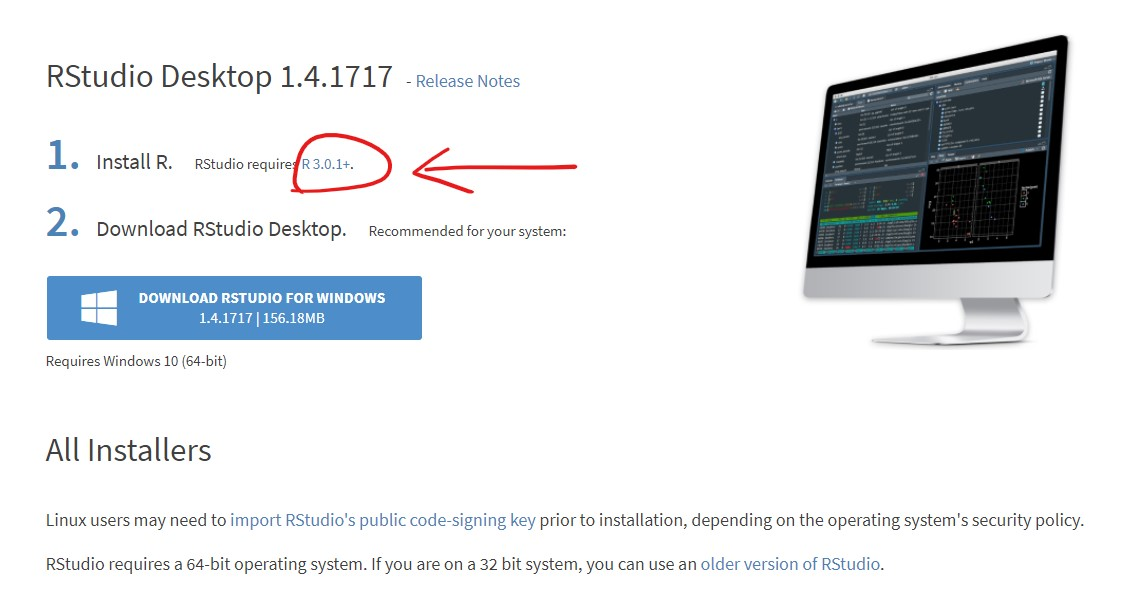
\includegraphics[width=6.25in,height=\textheight]{images/installr.jpg}}

\href{https://cran.rstudio.com/}{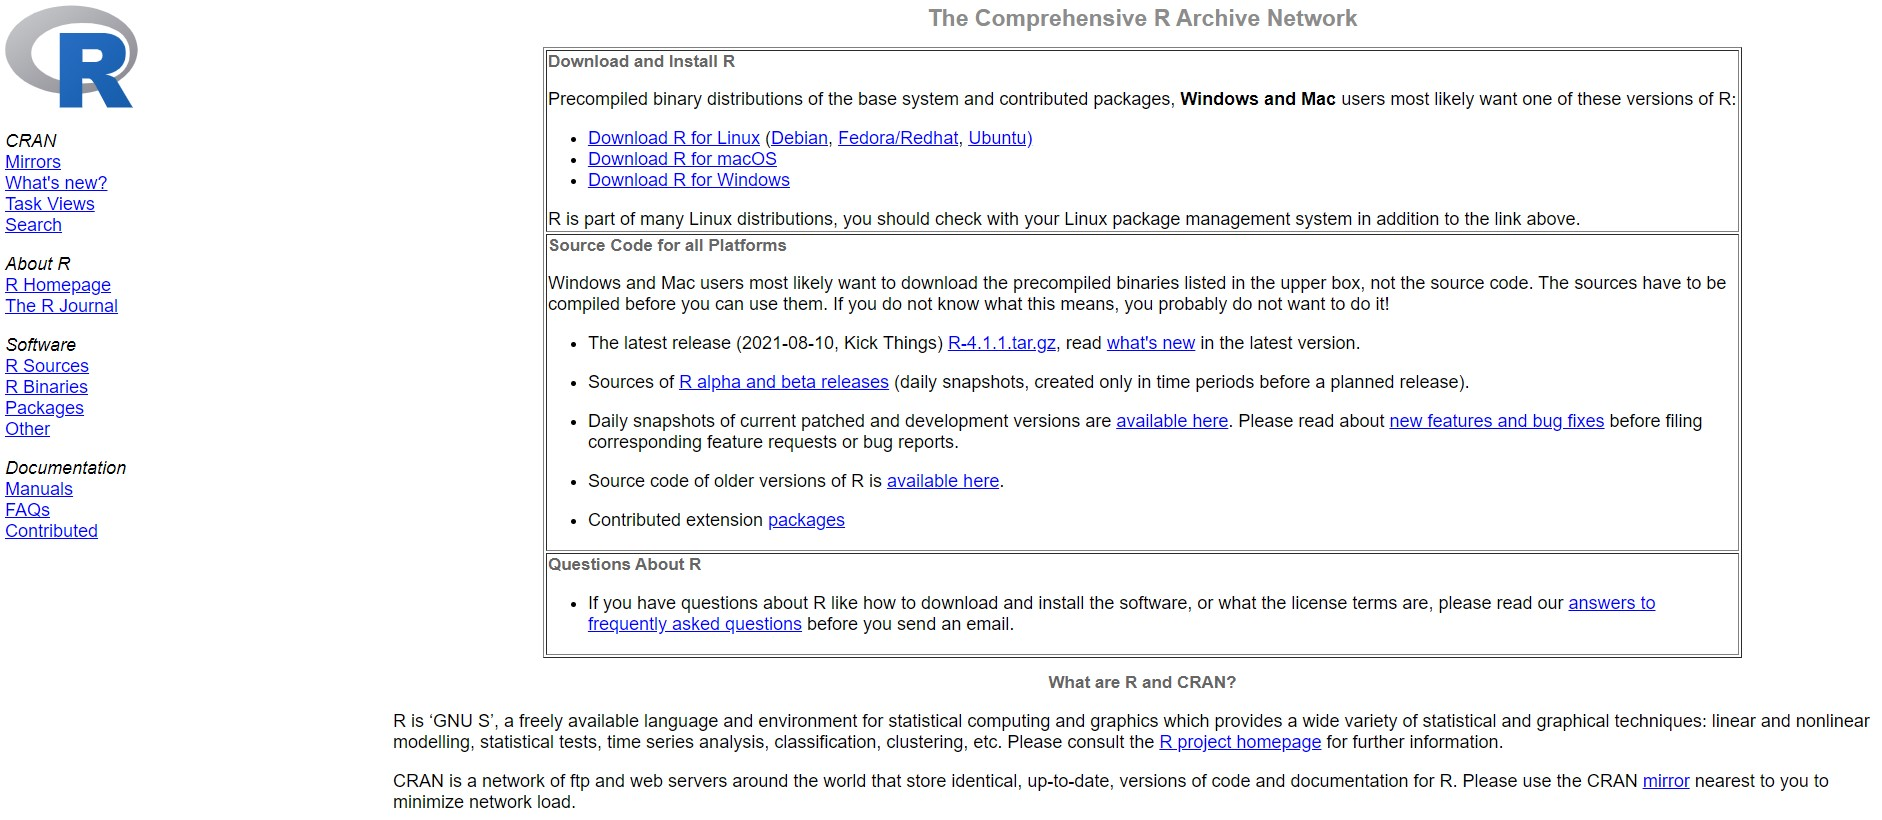
\includegraphics[width=6.25in,height=\textheight]{images/installr2.jpg}}

Run R's installer file after the downloading process is finished.
Next, we will also need the RStudio.

\href{https://www.rstudio.com/products/rstudio/download/\#download}{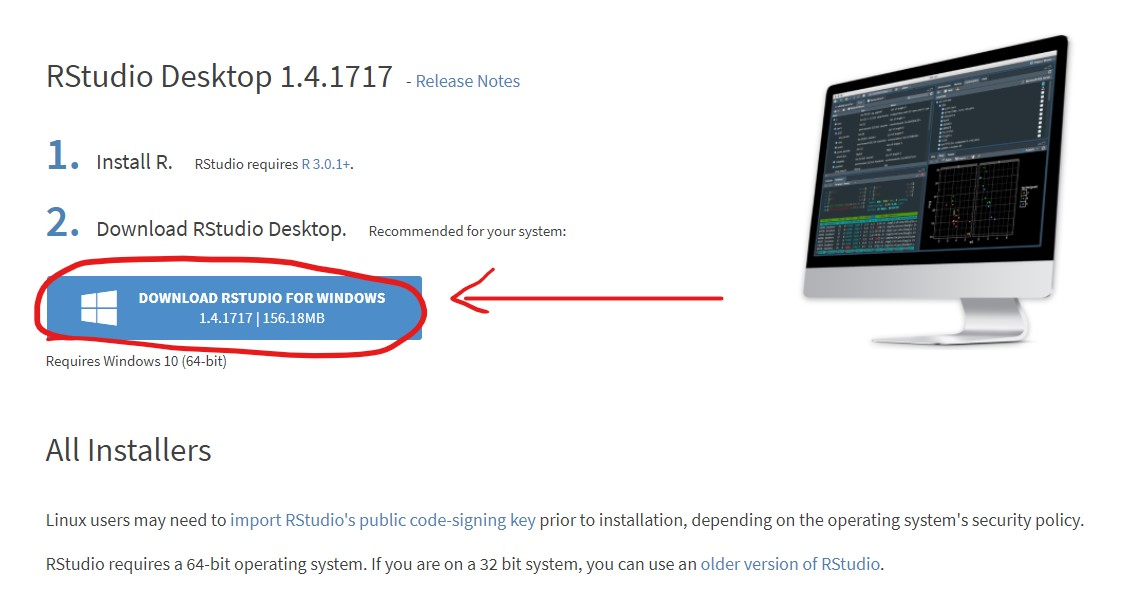
\includegraphics[width=6.25in,height=\textheight]{images/installr3.jpg}}

If the installation process of R and RStudio is finished, then we can open RStudio and start to learn the software.

\hypertarget{bootstrap}{%
\subsection{Bootstrap}\label{bootstrap}}

To continue your app customisation journey, you'll need to learn a little more about the \href{https://getbootstrap.com}{Bootstrap} framework used by Shiny.
Bootstrap is a collection of HTML conventions, CSS styles, and JS snippets bundled up into a convenient form.
Bootstrap grew out of a framework originally developed for Twitter and over the last 10 years has grown to become one of the most popular CSS frameworks used on the web.
Bootstrap is also popular in R --- you've undoubtedly seen many documents produced by \texttt{rmarkdown::html\_document()} and used many package websites made by \href{http://pkgdown.r-lib.org/}{pkgdown}, both of which also use Bootstrap.

As a Shiny developer, you don't need to think too much about Bootstrap, because Shiny functions automatically generate bootstrap compatible HTML for you.
But it's good to know that Bootstrap exists because then:

\begin{itemize}
\item
  You can use \texttt{bslib::bs\_theme()} to customise the visual appearance of your code, Section \ref{themes}.
\item
  You can use the \texttt{class} argument to customise some layouts, inputs, and outputs using Bootstrap class names, as you saw in Section \ref{action-buttons}.
\item
  You can make your own functions to generate Bootstrap components that Shiny doesn't provide, as explained in ``\href{https://rstudio.github.io/bslib/articles/theming.html\#utility-classes}{Utility classes}''.
\end{itemize}

It's also possible to use a completely different CSS framework.
A number of existing R packages make this easy by wrapping popular alternatives to Bootstrap:

\begin{itemize}
\item
  \href{https://appsilon.github.io/shiny.semantic/}{shiny.semantic}, by \href{https://appsilon.com/}{Appsilon}, builds on top of \href{https://fomantic-ui.com}{formantic UI}.
\item
  \href{https://github.com/RinteRface/shinyMobile}{shinyMobile}, by \href{https://rinterface.com}{RInterface}, builds on top of \href{https://framework7.io}{framework 7}, and is specifically designed for mobile apps.
\item
  \href{https://ericrayanderson.github.io/shinymaterial/}{shinymaterial}, by \href{https://github.com/ericrayanderson}{Eric Anderson}, is built on top of Google's \href{https://material.io/design}{Material design} framework.
\item
  \href{https://rstudio.github.io/shinydashboard/}{shinydashboard}, also by RStudio, provides a layout system designed to create dashboards.
\end{itemize}

You can find a fuller, and actively maintained, list at \url{https://github.com/nanxstats/awesome-shiny-extensions}.

\hypertarget{themes}{%
\subsection{Themes}\label{themes}}

Bootstrap is so ubiquitous within the R community that it's easy to get style fatigue: after a while every Shiny app and Rmd start to look the same.
The solution is theming with the \href{https://rstudio.github.io/bslib}{bslib} package.
bslib is relatively new package that allows you to override many Bootstrap defaults in order to create an appearance that is uniquely yours.
As I write this, bslib is mostly applicable only to Shiny, but work is afoot to bring its enhanced theming power to RMarkdown, pkgdown, and more.

If you're producing apps for your company, I highly recommend investing a little time in theming --- theming your app to match your corporate style guide is an easy way to make yourself look good.

\hypertarget{getting-started}{%
\subsubsection{Getting started}\label{getting-started}}

Create a theme with \texttt{bslib::bs\_theme()} then apply it to an app with the \texttt{theme} argument of the page layout function:

\begin{Shaded}
\begin{Highlighting}[]
\FunctionTok{fluidPage}\NormalTok{(}
  \AttributeTok{theme =}\NormalTok{ bslib}\SpecialCharTok{::}\FunctionTok{bs\_theme}\NormalTok{(...)}
\NormalTok{)}
\end{Highlighting}
\end{Shaded}

If not specified, Shiny will use the classic Bootstrap v3 theme that it has used basically since it was created.
By default, \texttt{bslib::bs\_theme()}, will use Bootstrap v4.
Using Bootstrap v4 instead of v3 will not cause problems if you only use built-in components.
There is a possibility that it might cause problems if you've used custom HTML, so you can force it to stay with v3 with \texttt{version\ =\ 3}.

\hypertarget{shiny-themes}{%
\subsubsection{Shiny themes}\label{shiny-themes}}

The easiest way to change the overall look of your app is to pick a premade ``\href{https://bootswatch.com}{bootswatch}'' theme using the \texttt{bootswatch} argument to \texttt{bslib::bs\_theme()}.
Figure \ref{fig:theme} shows the results of the following code, switching \texttt{"darkly"} out for other themes.

\hypertarget{part-week-2}{%
\part*{Week 2}\label{part-week-2}}
\addcontentsline{toc}{part}{Week 2}

\hypertarget{lecture2}{%
\section{Lecture 2}\label{lecture2}}

You can often make your app more usable by giving the user more insight into what is happening.
This might take the form of better messages when inputs don't make sense, or progress bars for operations that take a long time.
Some feedback occurs naturally through outputs, which you already know how to use, but you'll often need something else.
The goal of this chapter is to show you some of your other options.

We'll start with techniques for \textbf{validation}, informing the user when an input (or combination of inputs) is in an invalid state.
We'll then continue on to \textbf{notification}, sending general messages to the user, and \textbf{progress bars}, which give details for time consuming operations made up of many small steps.
We'll finish up by discussing dangerous actions, and how you give your users peace of mind with \textbf{confirmation} dialogs or the ability to \textbf{undo} an action.

\hypertarget{seminar2}{%
\section{Seminar 2}\label{seminar2}}

In this chapter, you'll learn how to wrap ggplot2 and dplyr function in a Shiny app.
(If you don't use the tidyverse, you can skip this chapter 😄.) The techniques for wrapping ggplot2 and dplyr functions in a functions and package, are a a little different and covered in other resources like \href{http://ggplot2.tidyverse.org/dev/articles/ggplot2-in-packages.html}{\emph{Using ggplot2 in packages}} or \href{http://dplyr.tidyverse.org/articles/programming.html}{\emph{Programming with dplyr}}.

\hypertarget{tidy-motivation}{%
\subsection{Motivation}\label{tidy-motivation}}

Imagine I want to create an app that allows you to filter a numeric variable to select rows that are greater than a threshold.
You might write something like this:

Let's begin with this call to \texttt{filter()} which uses a data-variable (\texttt{carat}) and an env-variable (\texttt{min}):

\begin{Shaded}
\begin{Highlighting}[]
\FunctionTok{ggplot}\NormalTok{(cars, }\FunctionTok{aes}\NormalTok{(speed, dist)) }\SpecialCharTok{+} 
  \FunctionTok{geom\_point}\NormalTok{()}
\end{Highlighting}
\end{Shaded}

\begin{center}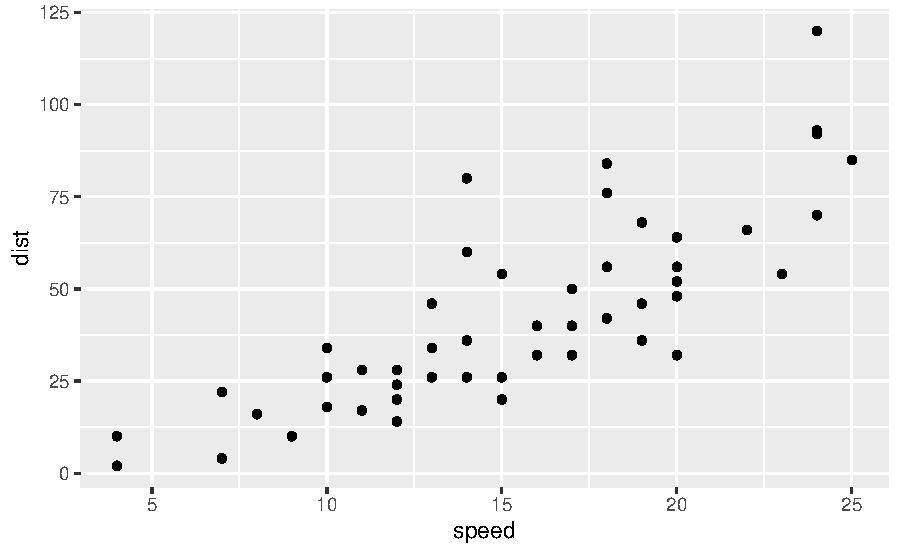
\includegraphics[width=0.7\linewidth]{Data-Analysis-Coursebook_files/figure-latex/unnamed-chunk-4-1} \end{center}

\hypertarget{part-week-3}{%
\part*{Week 3}\label{part-week-3}}
\addcontentsline{toc}{part}{Week 3}

\hypertarget{lecture3}{%
\section{Lecture 3}\label{lecture3}}

You can often make your app more usable by giving the user more insight into what is happening.
This might take the form of better messages when inputs don't make sense, or progress bars for operations that take a long time.
Some feedback occurs naturally through outputs, which you already know how to use, but you'll often need something else.
The goal of this chapter is to show you some of your other options.

We'll start with techniques for \textbf{validation}, informing the user when an input (or combination of inputs) is in an invalid state.
We'll then continue on to \textbf{notification}, sending general messages to the user, and \textbf{progress bars}, which give details for time consuming operations made up of many small steps.
We'll finish up by discussing dangerous actions, and how you give your users peace of mind with \textbf{confirmation} dialogs or the ability to \textbf{undo} an action.

\hypertarget{seminar3}{%
\section{Seminar 3}\label{seminar3}}

Transferring files to and from the user is a common feature of apps.
You can use it to upload data for analysis, or download the results as a dataset or as a report.
This chapter shows the UI and server components that you'll need to transfer files in and out of your app.

\hypertarget{upload}{%
\subsection{Upload}\label{upload}}

We'll start by discussing file uploads, showing you the basic UI and server components, and then showing how they fit together in a simple app.

\hypertarget{ui}{%
\subsubsection{UI}\label{ui}}

\hypertarget{part-week-4}{%
\part*{Week 4}\label{part-week-4}}
\addcontentsline{toc}{part}{Week 4}

\hypertarget{lecture4}{%
\section{Lecture 4}\label{lecture4}}

In this chapter, you'll learn how to wrap ggplot2 and dplyr function in a Shiny app.
(If you don't use the tidyverse, you can skip this chapter 😄.) The techniques for wrapping ggplot2 and dplyr functions in a functions and package, are a a little different and covered in other resources like \href{http://ggplot2.tidyverse.org/dev/articles/ggplot2-in-packages.html}{\emph{Using ggplot2 in packages}} or \href{http://dplyr.tidyverse.org/articles/programming.html}{\emph{Programming with dplyr}}.

\hypertarget{tidy-motivation}{%
\subsection{Motivation}\label{tidy-motivation}}

Imagine I want to create an app that allows you to filter a numeric variable to select rows that are greater than a threshold.
You might write something like this:

Let's begin with this call to \texttt{filter()} which uses a data-variable (\texttt{carat}) and an env-variable (\texttt{min}):

\begin{Shaded}
\begin{Highlighting}[]
\FunctionTok{ggplot}\NormalTok{(cars, }\FunctionTok{aes}\NormalTok{(speed, dist)) }\SpecialCharTok{+} 
  \FunctionTok{geom\_point}\NormalTok{()}
\end{Highlighting}
\end{Shaded}

\begin{center}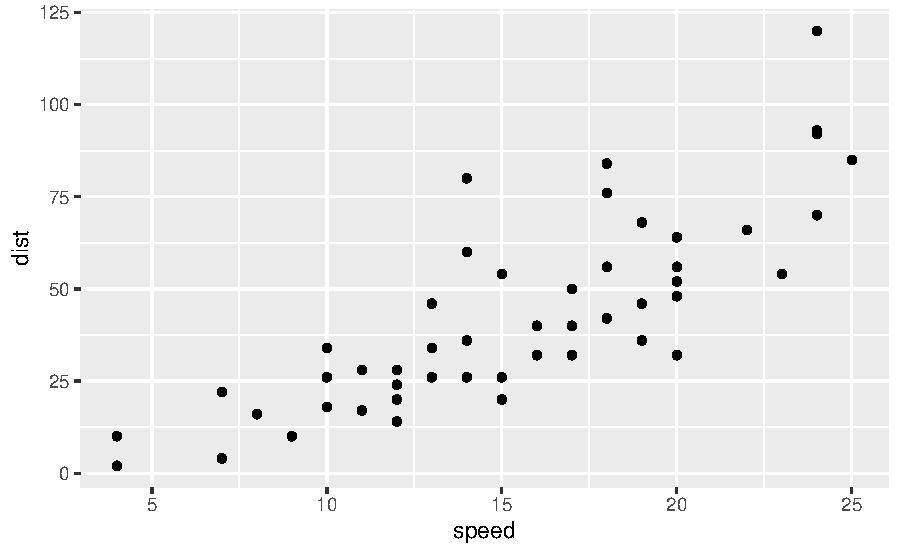
\includegraphics[width=0.7\linewidth]{Data-Analysis-Coursebook_files/figure-latex/unnamed-chunk-5-1} \end{center}

\hypertarget{seminar4}{%
\section{Ggplot}\label{seminar4}}

\hypertarget{motivuxe1ciuxf3-a-ggplot-package-hasznuxe1latuxe1hoz}{%
\subsection{Motiváció a ggplot package használatához}\label{motivuxe1ciuxf3-a-ggplot-package-hasznuxe1latuxe1hoz}}

Bár maga a base R {[}értve itt ilyenkor mindig a \texttt{plot} paranccsal készült ábrákat{]} segítségével is lehet ábrákat készíteni, ez az egyszerűségét leszámítva nagyon ritkán ajánlott. Helyette érdemes a ggplot2-t alkalmazni, amely bár komplexebb, mint a base R, a személyre szabhatóságának szinte nincs felső határa.

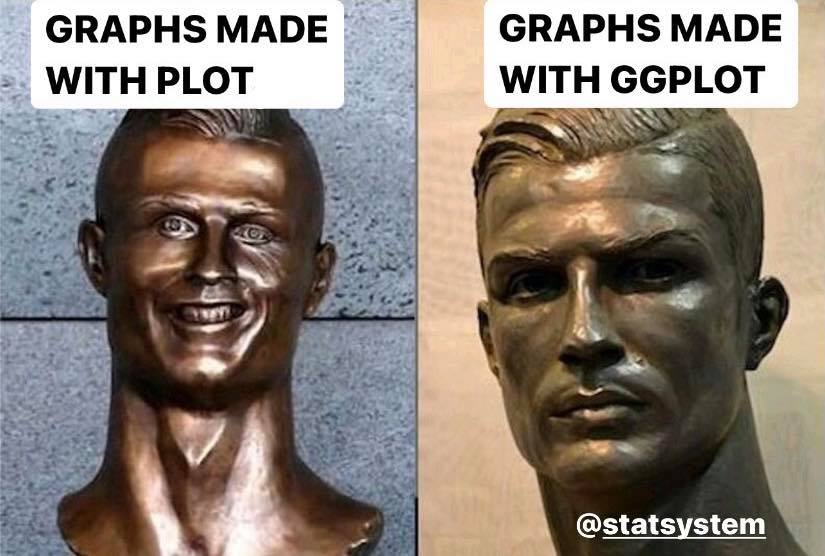
\includegraphics[width=4.16667in,height=\textheight]{images/plot_ggplot.jpg}

Ám amelett, hogy szebb ábráink lesznek van egy sokkal fontosabb ok, amiért a ggplotot használjuk. A csomag a nevét Leland Wilkinson \textbf{Grammar of Graphics} c.~munkája után kapta (innen a \emph{gg}), amelyben megfogalmazásra került lényegében az ideális ábrakészítő algoritmus struktúrája. Mivel a ggplot2 ezt az elvet követi, így meglátjátok majd, hogy bár sok dolgot kell fejben tartani, minden logikus benne. Miután sikerül elsajátítani ezt az anyagot (és némi utána olvasás után) bármilyen szükséges ábrát el fogtok tudni készíteni.

\hypertarget{bevezetuxe9s}{%
\subsection{Bevezetés}\label{bevezetuxe9s}}

A ggplot2 telepíthető önállóan is, illetve ez a csomag része egy ``csomaggyűjteménynek'', amit \texttt{tidyverse}-nek hívnak. Jelenleg mi csak a ggplot2-vel fogunk foglalkozni, így annak telepítése és betöltése is bőven elegendő lesz. Így annak függvényébne, hogy le van-e már töltve a package telepítsük {[}\texttt{install.packages("ggplot2")}{]}, vagy ne, majd töltsük be {[}\texttt{library(ggplot2)}{]}. A ggplot2 helyett lehet egyből a \texttt{tidyverse}-t is betölteni, azonban jelenleg a többi package redundáns nekünk.

\begin{Shaded}
\begin{Highlighting}[]
\FunctionTok{library}\NormalTok{(ggplot2)}
\end{Highlighting}
\end{Shaded}

A ggplot2-vel kapunk néhány kiegészítő adattáblát, az egyszerűség kedvéért használjuk most ezek közül a \texttt{diamonds}-t. Pillanatra tekintsük meg az adattábla felépítését:

\begin{Shaded}
\begin{Highlighting}[]
\FunctionTok{head}\NormalTok{(diamonds)}
\end{Highlighting}
\end{Shaded}

\begin{verbatim}
#> Error in tab_header(., "A diamonds adattábla"): could not find function "tab_header"
\end{verbatim}

Lássuk az első ábránkat ggplottal!

\begin{Shaded}
\begin{Highlighting}[]
\FunctionTok{ggplot}\NormalTok{(}\AttributeTok{data =}\NormalTok{ diamonds, }\AttributeTok{mapping =} \FunctionTok{aes}\NormalTok{(}\AttributeTok{x =}\NormalTok{ carat, }\AttributeTok{y =}\NormalTok{ price)) }\SpecialCharTok{+}
  \FunctionTok{geom\_point}\NormalTok{()}
\end{Highlighting}
\end{Shaded}

\begin{figure}

{\centering 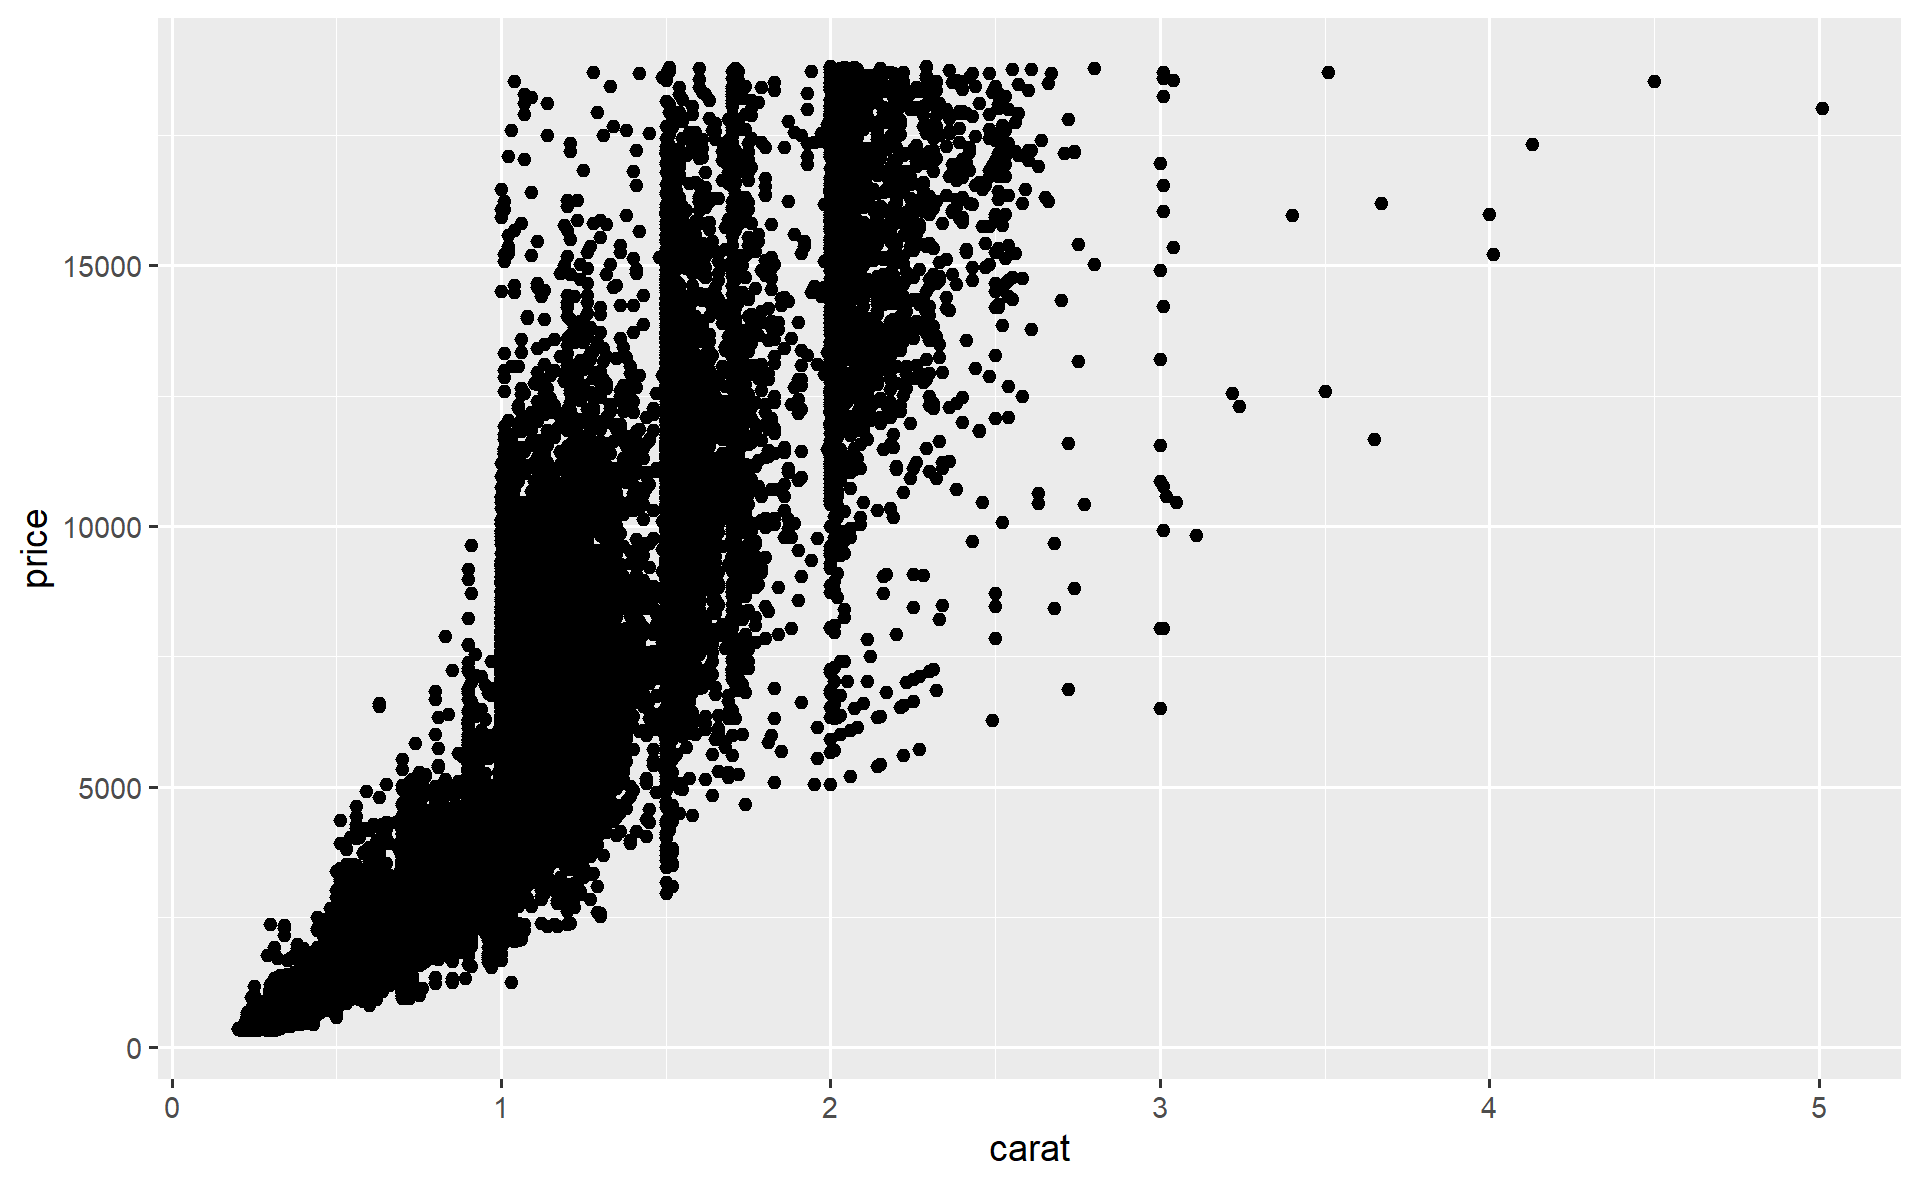
\includegraphics[width=0.7\linewidth]{Data-Analysis-Coursebook_files/figure-latex/unnamed-chunk-9-1} 

}

\caption{A legelső ábránk ggplot használatával}\label{fig:unnamed-chunk-9}
\end{figure}

Amit látunk, hogy az ábrázolás a \texttt{ggplot} paranccsal kezdődik. Itt definiálni kell, hogy melyik táblának adatait szeretnénk felhasználni (\texttt{diamonds}), majd pedig az ábrázoláshoz használt ``keretet'', ami az \texttt{aes}-es belül kap helyet. Itt általában (mint például most) az x és y tengelyen ábrázolt adatokat kell megadni. A ggplot-ot mindig egy \texttt{geom} parancs követi, amellyel az ábra típusát adjuk meg.

Ezen az ábrán azonban még nicsen semmilyen felirat. Minden felirat megadható a \texttt{labs()} függvényben. Példa:

\begin{Shaded}
\begin{Highlighting}[]
\FunctionTok{ggplot}\NormalTok{(}\AttributeTok{data =}\NormalTok{ diamonds, }\AttributeTok{mapping =} \FunctionTok{aes}\NormalTok{(}\AttributeTok{x =}\NormalTok{ carat, }\AttributeTok{y =}\NormalTok{ price)) }\SpecialCharTok{+}
  \FunctionTok{geom\_point}\NormalTok{() }\SpecialCharTok{+}
  \FunctionTok{labs}\NormalTok{(}
    \AttributeTok{title =} \StringTok{"Figyelemfelkeltő cím"}\NormalTok{,}
    \AttributeTok{subtitle =} \StringTok{"Az alcím pontosítja a témát"}\NormalTok{,}
    \AttributeTok{x =} \StringTok{"x{-}tengely váltózójának neve"}\NormalTok{,}
    \AttributeTok{y =} \StringTok{"y{-}tengely változójának neve"}\NormalTok{,}
    \AttributeTok{caption =} \StringTok{"Mindent megmagyarázó hosszú leírás."}
\NormalTok{  )}
\end{Highlighting}
\end{Shaded}

\begin{figure}

{\centering 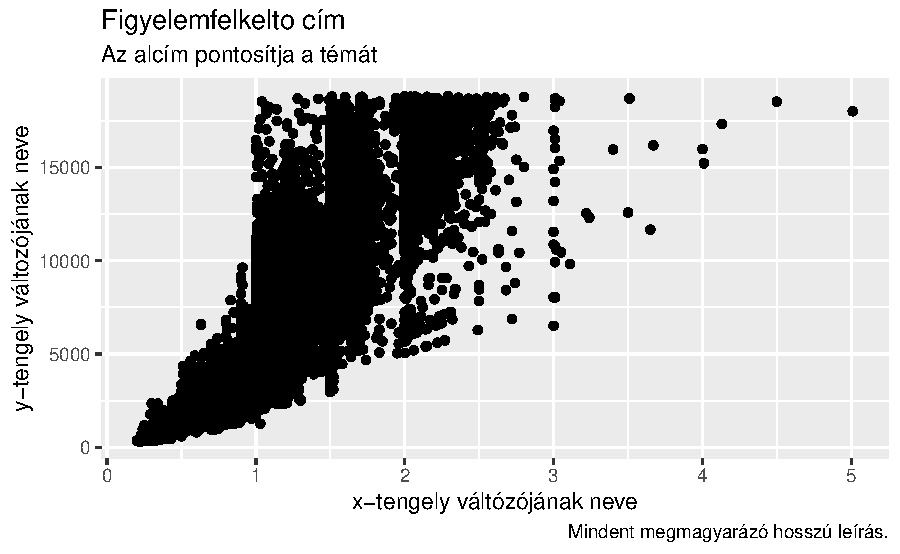
\includegraphics[width=0.7\linewidth]{Data-Analysis-Coursebook_files/figure-latex/unnamed-chunk-10-1} 

}

\caption{Feliratok elhelyezése az ábrán}\label{fig:unnamed-chunk-10}
\end{figure}

\hypertarget{esquisse}{%
\subsection{Esquisse}\label{esquisse}}

Első látásra ez még lehet túl sok információ, illetve a következőkben a bonyolultabb ábrákra rátérve elveszítheti az ember a fonalat. Amíg bizonytalan a ggplot használata javaslom a \texttt{esquisse} packaget Ezt csupán telepíteni kell a \texttt{install.packages("esquisse")} paranccsal, majd az \texttt{Addins} menüből lehet előhívni. Ennek segítségével ``manuálisan'' adhatóak meg az ábra elemei. Lássuk például az előző ábrát!

\hypertarget{szuxedn}{%
\subsection{Szín}\label{szuxedn}}

Az \texttt{esquisse} automatikusan hozzáadott 3 elemet, amit akkor itt tisztázni szükséges. A \texttt{geom} függvényen belül a \texttt{size} paraméter a pontok méretért felel, míg a \texttt{color} a pontok színéért. Színként megadható bármilyen hexadecimális érték, illetve az R számos színt ismer (\texttt{red}, \texttt{green}, \texttt{blue}, \texttt{black}, stb.).

\begin{verbatim}
#> Error in include_graphics("images/color_examples.png"): could not find function "include_graphics"
\end{verbatim}

\hypertarget{tuxe9ma}{%
\subsection{Téma}\label{tuxe9ma}}

A 3. dolog amit \texttt{esquisse} csatolt a kódunk mellé az egy \texttt{theme} parancs. Ez a parancstípus az ábra hátterének, jelmagyarázatának és feliratainak esztétikáját adja meg. Lássunk ezekből is néhányat!

\begin{Shaded}
\begin{Highlighting}[]
\FunctionTok{ggplot}\NormalTok{(}\AttributeTok{data =}\NormalTok{ diamonds, }\AttributeTok{mapping =} \FunctionTok{aes}\NormalTok{(}\AttributeTok{x =}\NormalTok{ carat, }\AttributeTok{y =}\NormalTok{ price)) }\SpecialCharTok{+}
  \FunctionTok{geom\_point}\NormalTok{() }\SpecialCharTok{+}
  \FunctionTok{theme\_bw}\NormalTok{()}

\FunctionTok{ggplot}\NormalTok{(}\AttributeTok{data =}\NormalTok{ diamonds, }\AttributeTok{mapping =} \FunctionTok{aes}\NormalTok{(}\AttributeTok{x =}\NormalTok{ carat, }\AttributeTok{y =}\NormalTok{ price)) }\SpecialCharTok{+}
  \FunctionTok{geom\_point}\NormalTok{() }\SpecialCharTok{+}
  \FunctionTok{theme\_classic}\NormalTok{()}

\FunctionTok{ggplot}\NormalTok{(}\AttributeTok{data =}\NormalTok{ diamonds, }\AttributeTok{mapping =} \FunctionTok{aes}\NormalTok{(}\AttributeTok{x =}\NormalTok{ carat, }\AttributeTok{y =}\NormalTok{ price)) }\SpecialCharTok{+}
  \FunctionTok{geom\_point}\NormalTok{() }\SpecialCharTok{+}
  \FunctionTok{theme\_grey}\NormalTok{()}

\FunctionTok{ggplot}\NormalTok{(}\AttributeTok{data =}\NormalTok{ diamonds, }\AttributeTok{mapping =} \FunctionTok{aes}\NormalTok{(}\AttributeTok{x =}\NormalTok{ carat, }\AttributeTok{y =}\NormalTok{ price)) }\SpecialCharTok{+}
  \FunctionTok{geom\_point}\NormalTok{() }\SpecialCharTok{+}
  \FunctionTok{theme\_minimal}\NormalTok{()}
\end{Highlighting}
\end{Shaded}

\begin{verbatim}
#> Error: Can't add `(p + theme_classic() + ggtitle("theme_classic"))` to a ggplot object.
\end{verbatim}

Persze van még rengeteg, válogass nyugodtan: \url{https://www.datanovia.com/en/blog/ggplot-themes-gallery/}

Ami még fontos, hogy a \texttt{theme()} függvénnyel módosíthatóak a témánk egyes elemei (háttérszín, betűszín stb.). Például legyen tényleg figyelemfelkeltő a fentebb bemutatott cím!

\begin{Shaded}
\begin{Highlighting}[]
\FunctionTok{ggplot}\NormalTok{(}\AttributeTok{data =}\NormalTok{ diamonds, }\AttributeTok{mapping =} \FunctionTok{aes}\NormalTok{(}\AttributeTok{x =}\NormalTok{ carat, }\AttributeTok{y =}\NormalTok{ price)) }\SpecialCharTok{+}
  \FunctionTok{geom\_point}\NormalTok{() }\SpecialCharTok{+}
  \FunctionTok{labs}\NormalTok{(}
    \AttributeTok{title =} \StringTok{"Figyelemfelkeltő cím"}\NormalTok{,}
    \AttributeTok{subtitle =} \StringTok{"Az alcím pontosítja a témát"}\NormalTok{,}
    \AttributeTok{x =} \StringTok{"x{-}tengely váltózójának neve"}\NormalTok{,}
    \AttributeTok{y =} \StringTok{"y{-}tengely változójának neve"}\NormalTok{,}
    \AttributeTok{caption =} \StringTok{"Mindent megmagyarázó hosszú leírás."}
\NormalTok{  ) }\SpecialCharTok{+} 
  \FunctionTok{theme}\NormalTok{(}
    \AttributeTok{plot.title =} \FunctionTok{element\_text}\NormalTok{(}\AttributeTok{color =} \StringTok{"red"}\NormalTok{, }\AttributeTok{size =} \DecValTok{30}\NormalTok{)}
\NormalTok{  )}
\end{Highlighting}
\end{Shaded}

\begin{figure}

{\centering 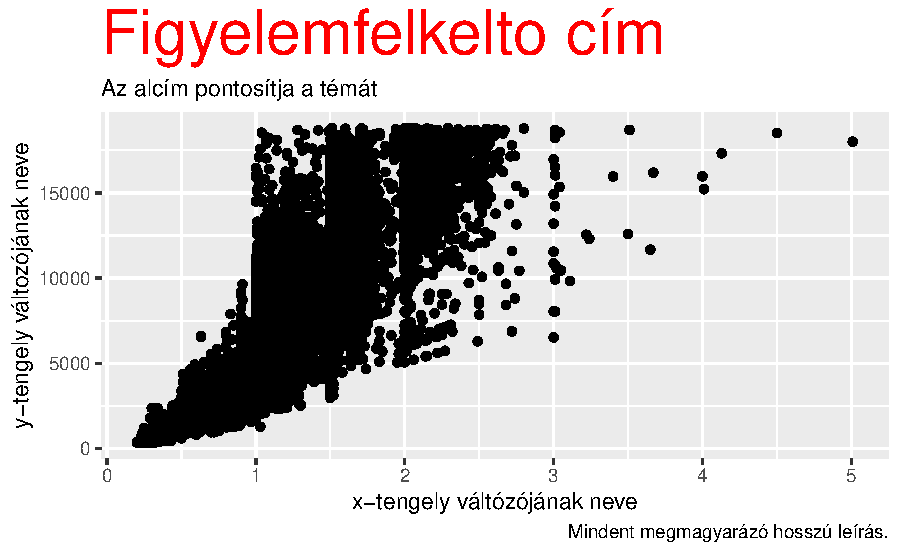
\includegraphics[width=0.7\linewidth]{Data-Analysis-Coursebook_files/figure-latex/unnamed-chunk-16-1} 

}

\caption{Téma egy elmének megváltoztatására példa}\label{fig:unnamed-chunk-16}
\end{figure}

\hypertarget{geom}{%
\subsection{Geom}\label{geom}}

A plot szempontjából lényeges fontosabb azonban a \texttt{geom} függvény. Maga a függvény adja meg az ábra típusát, azonban a benne foglalt paraméterek sem elhanyagolhatóak. Nézzük példát a típusokra (csak párat van módom említeni a végtelenül sokból)!

\begin{Shaded}
\begin{Highlighting}[]
\FunctionTok{ggplot}\NormalTok{(}\AttributeTok{data =}\NormalTok{ diamonds, }\AttributeTok{mapping =} \FunctionTok{aes}\NormalTok{(}\AttributeTok{x =}\NormalTok{ carat)) }\SpecialCharTok{+}
  \FunctionTok{geom\_histogram}\NormalTok{()}

\FunctionTok{ggplot}\NormalTok{(}\AttributeTok{data =}\NormalTok{ diamonds, }\AttributeTok{mapping =} \FunctionTok{aes}\NormalTok{(}\AttributeTok{x =}\NormalTok{ carat)) }\SpecialCharTok{+}
  \FunctionTok{geom\_histogram}\NormalTok{() }\SpecialCharTok{+} 
  \FunctionTok{geom\_vline}\NormalTok{(}\AttributeTok{xintercept =} \FunctionTok{mean}\NormalTok{(diamonds}\SpecialCharTok{$}\NormalTok{carat), }\AttributeTok{color =} \StringTok{\textquotesingle{}red4\textquotesingle{}}\NormalTok{)}

\FunctionTok{ggplot}\NormalTok{(}\AttributeTok{data =}\NormalTok{ diamonds, }\AttributeTok{mapping =} \FunctionTok{aes}\NormalTok{(}\AttributeTok{x =}\NormalTok{ cut)) }\SpecialCharTok{+}
  \FunctionTok{geom\_bar}\NormalTok{()}

\FunctionTok{ggplot}\NormalTok{(}\AttributeTok{data =}\NormalTok{ diamonds, }\AttributeTok{mapping =} \FunctionTok{aes}\NormalTok{(}\AttributeTok{x =}\NormalTok{ carat, }\AttributeTok{y =}\NormalTok{ price)) }\SpecialCharTok{+}
  \FunctionTok{geom\_point}\NormalTok{()}
\end{Highlighting}
\end{Shaded}

\begin{verbatim}
#> Error: Can't add `ggplot(data = diamonds, mapping = aes(x = carat))` to a ggplot object.
\end{verbatim}

A 2. kódból látszik, hogy több \texttt{geom} is tartozhat egyszerre egy ábrához, így lehet például egy hisztogramon feltüntetni az átlagot egy függőleges vonallal (\texttt{geom\_vline}). Ennek párja is rendkívül hasznos tud lennni a \texttt{geom\_hline}, amivel lehet akár 0 mentén húzni egy vízszintes vonalat. A \texttt{cut} egy kategorikus változó az adattáblánkban, amelynek az egyes kategóriákhoz tartozó darabszámait egy \texttt{geom\_bar}-al gyorsan kirajzolhatjuk. Most nézzük a paramétereket! Eddig láttunk példát a \texttt{size}-ra és a \texttt{color}-ra, ami majdnem minden geom esetén csinál valamit, de egyes geomoknak vannak speciális paramétereik is, mint pélául az előbbi példában az \texttt{xintercept}. Lássunk néhány további fontos paraméterre példákat:

\begin{verbatim}
#> Error in cols_align(., align = "center"): could not find function "cols_align"
\end{verbatim}

\begin{Shaded}
\begin{Highlighting}[]
\FunctionTok{ggplot}\NormalTok{(}\AttributeTok{data =}\NormalTok{ diamonds, }\AttributeTok{mapping =} \FunctionTok{aes}\NormalTok{(}\AttributeTok{x =}\NormalTok{ carat)) }\SpecialCharTok{+}
  \FunctionTok{geom\_histogram}\NormalTok{(}\AttributeTok{color =} \StringTok{\textquotesingle{}black\textquotesingle{}}\NormalTok{, }\AttributeTok{fill =} \StringTok{"red"}\NormalTok{)}

\FunctionTok{ggplot}\NormalTok{(}\AttributeTok{data =}\NormalTok{ diamonds, }\AttributeTok{mapping =} \FunctionTok{aes}\NormalTok{(}\AttributeTok{x =}\NormalTok{ carat)) }\SpecialCharTok{+}
  \FunctionTok{geom\_vline}\NormalTok{(}\AttributeTok{xintercept =} \FunctionTok{mean}\NormalTok{(diamonds}\SpecialCharTok{$}\NormalTok{carat), }\AttributeTok{lty =} \DecValTok{2}\NormalTok{)}

\FunctionTok{ggplot}\NormalTok{(}\AttributeTok{data =}\NormalTok{ diamonds, }\AttributeTok{mapping =} \FunctionTok{aes}\NormalTok{(}\AttributeTok{x =}\NormalTok{ cut)) }\SpecialCharTok{+}
  \FunctionTok{geom\_bar}\NormalTok{(}\AttributeTok{alpha =}\NormalTok{ .}\DecValTok{3}\NormalTok{)}

\FunctionTok{ggplot}\NormalTok{(}\AttributeTok{data =}\NormalTok{ diamonds, }\AttributeTok{mapping =} \FunctionTok{aes}\NormalTok{(}\AttributeTok{x =}\NormalTok{ carat, }\AttributeTok{y =}\NormalTok{ price)) }\SpecialCharTok{+}
  \FunctionTok{geom\_point}\NormalTok{(}\AttributeTok{shape =} \DecValTok{21}\NormalTok{, }\AttributeTok{color =} \StringTok{\textquotesingle{}black\textquotesingle{}}\NormalTok{, }\AttributeTok{fill =} \StringTok{\textquotesingle{}green\textquotesingle{}}\NormalTok{)}
\end{Highlighting}
\end{Shaded}

\begin{verbatim}
#> Error: Can't add `ggplot(data = diamonds, mapping = aes(x = carat))` to a ggplot object.
\end{verbatim}

Az utolsó ábra itt még igényel némi magyarázatot. A pont diagram alapbeállítása szerint csak \texttt{color} paraméter adható meg. Azonban ha a \texttt{shape}-t átállítjuk, akkor van lehetőségünk olyan pontdiagramokat rajzolni, amelyeknek belsejéhez tartozó színt adja meg a \texttt{fill}, a szegélyét a \texttt{color}.

\hypertarget{aes}{%
\subsection{Aes}\label{aes}}

Korábban csak átsiklottunk az \texttt{aes()} függvényen, ami az ábra ``keretét'' adta. Most nézzük meg kicsit részletesebben! A \texttt{mapping} paraméter, aminek megadásához használjuk fel az \texttt{aes()}-t az előzőekben a \texttt{ggplot()} függvényen belül szerepelt. Ennek azonban nem kell feltétlenül így lennie. A következő 3 kód, mind ugyanazt hajtja végre (erre még visszatérünk):

\begin{Shaded}
\begin{Highlighting}[]
\FunctionTok{ggplot}\NormalTok{(diamonds, }\FunctionTok{aes}\NormalTok{(}\AttributeTok{x =}\NormalTok{ carat, }\AttributeTok{y =}\NormalTok{ price)) }\SpecialCharTok{+}
  \FunctionTok{geom\_point}\NormalTok{()}

\FunctionTok{ggplot}\NormalTok{(diamonds) }\SpecialCharTok{+}
  \FunctionTok{aes}\NormalTok{(}\AttributeTok{x =}\NormalTok{ carat, }\AttributeTok{y =}\NormalTok{ price) }\SpecialCharTok{+}
  \FunctionTok{geom\_point}\NormalTok{()}

\FunctionTok{ggplot}\NormalTok{(diamonds) }\SpecialCharTok{+}
  \FunctionTok{geom\_point}\NormalTok{(}\FunctionTok{aes}\NormalTok{(}\AttributeTok{x =}\NormalTok{ carat, }\AttributeTok{y =}\NormalTok{ price))}
\end{Highlighting}
\end{Shaded}

Az \texttt{aes}-ben azonban nem csak x- és y-tengely változóit definiálhatjuk. Minden ami \texttt{geom}-beni paraméter, az megadásra kerülhet az \texttt{aes()}-ben is, azonban ilyenkor az adott változó értéke szerint kerül megadásra (pl.: egy harmadik változó szerint van definiálva a méret, vagy a szín). Ami paraméter az \texttt{aes()}-ben kerül megadásra, az automatikusan a jelmagyarázatra is felkerül. Lássunk két példát!

\begin{Shaded}
\begin{Highlighting}[]
\FunctionTok{ggplot}\NormalTok{(diamonds, }\FunctionTok{aes}\NormalTok{(}\AttributeTok{x =}\NormalTok{ carat, }\AttributeTok{y =}\NormalTok{ price, }\AttributeTok{color =}\NormalTok{ cut)) }\SpecialCharTok{+}
  \FunctionTok{geom\_point}\NormalTok{()}

\FunctionTok{ggplot}\NormalTok{(diamonds, }\FunctionTok{aes}\NormalTok{(}\AttributeTok{x =}\NormalTok{ carat, }\AttributeTok{y =}\NormalTok{ price, }\AttributeTok{size =}\NormalTok{ cut)) }\SpecialCharTok{+}
  \FunctionTok{geom\_point}\NormalTok{(}\AttributeTok{alpha =}\NormalTok{ .}\DecValTok{3}\NormalTok{)}
\end{Highlighting}
\end{Shaded}

\begin{verbatim}
#> Error in (ggplot(diamonds, aes(x = carat, y = price, color = cut)) + geom_point())/(ggplot(diamonds, : non-numeric argument to binary operator
\end{verbatim}

Ha egy változó szerint adjuk meg a színeket, akkor érdemes a színezésnek módját is megadni. Erre leginkább a \texttt{viridis} függvények a javasoltak (számos alkalommla láthatod tudományos publikációkban + \emph{végződésre figyeljünk: viridis\_d, mint diszkért/viridis\_c, mint folytonos}), de ha például fontos, hogy fekete-fehér legyen, arra is van mód, illetve ``kézileg'' is meg lehet adni színeket.

\begin{Shaded}
\begin{Highlighting}[]
\FunctionTok{ggplot}\NormalTok{(diamonds, }\FunctionTok{aes}\NormalTok{(}\AttributeTok{x =}\NormalTok{ carat, }\AttributeTok{y =}\NormalTok{ price, }\AttributeTok{color =}\NormalTok{ cut)) }\SpecialCharTok{+}
  \FunctionTok{geom\_point}\NormalTok{()}

\FunctionTok{ggplot}\NormalTok{(diamonds, }\FunctionTok{aes}\NormalTok{(}\AttributeTok{x =}\NormalTok{ carat, }\AttributeTok{y =}\NormalTok{ price, }\AttributeTok{color =}\NormalTok{ cut)) }\SpecialCharTok{+}
  \FunctionTok{geom\_point}\NormalTok{() }\SpecialCharTok{+}
  \FunctionTok{scale\_color\_viridis\_d}\NormalTok{(}\AttributeTok{option =} \StringTok{"magma"}\NormalTok{)}

\FunctionTok{ggplot}\NormalTok{(diamonds, }\FunctionTok{aes}\NormalTok{(}\AttributeTok{x =}\NormalTok{ carat, }\AttributeTok{y =}\NormalTok{ price, }\AttributeTok{color =}\NormalTok{ cut)) }\SpecialCharTok{+}
  \FunctionTok{geom\_point}\NormalTok{() }\SpecialCharTok{+} 
  \FunctionTok{scale\_color\_manual}\NormalTok{(}
    \AttributeTok{values =} \FunctionTok{c}\NormalTok{(}\StringTok{"red"}\NormalTok{, }\StringTok{"green"}\NormalTok{, }\StringTok{"blue"}\NormalTok{, }\StringTok{"yellow"}\NormalTok{, }\StringTok{"orange"}\NormalTok{)}
\NormalTok{    )}
\end{Highlighting}
\end{Shaded}

\begin{verbatim}
#> Error in (ggplot(diamonds, aes(x = carat, y = price, color = cut)) + geom_point())/(ggplot(diamonds, : non-numeric argument to binary operator
\end{verbatim}

És most vissza oda, hogy miért is hasznos, hogy több \texttt{aes()} definiálható egyetlen ábrán. Elképzelhető, hogy két külön \texttt{geom}-ot használunk együtt. Legyen mondjuk egy pontdiagram és egy azokra illesztett ``trendvonal''. Utóbbi a \texttt{geom\_smooth} paranccsal érhető el, s amennyiben lineáris függvény formára vágyunk (yes), úgy adjuk meg neki a \texttt{method\ =\ "lm"} paramétert.

\begin{Shaded}
\begin{Highlighting}[]
\FunctionTok{ggplot}\NormalTok{(diamonds, }\FunctionTok{aes}\NormalTok{(}\AttributeTok{x =}\NormalTok{ carat, }\AttributeTok{y =}\NormalTok{ price, }\AttributeTok{color =}\NormalTok{ cut)) }\SpecialCharTok{+}
  \FunctionTok{geom\_point}\NormalTok{() }\SpecialCharTok{+} 
  \FunctionTok{geom\_smooth}\NormalTok{(}\AttributeTok{method =} \StringTok{"lm"}\NormalTok{)}
\CommentTok{\#\textgreater{} \textasciigrave{}geom\_smooth()\textasciigrave{} using formula \textquotesingle{}y \textasciitilde{} x\textquotesingle{}}
\end{Highlighting}
\end{Shaded}

\begin{figure}

{\centering 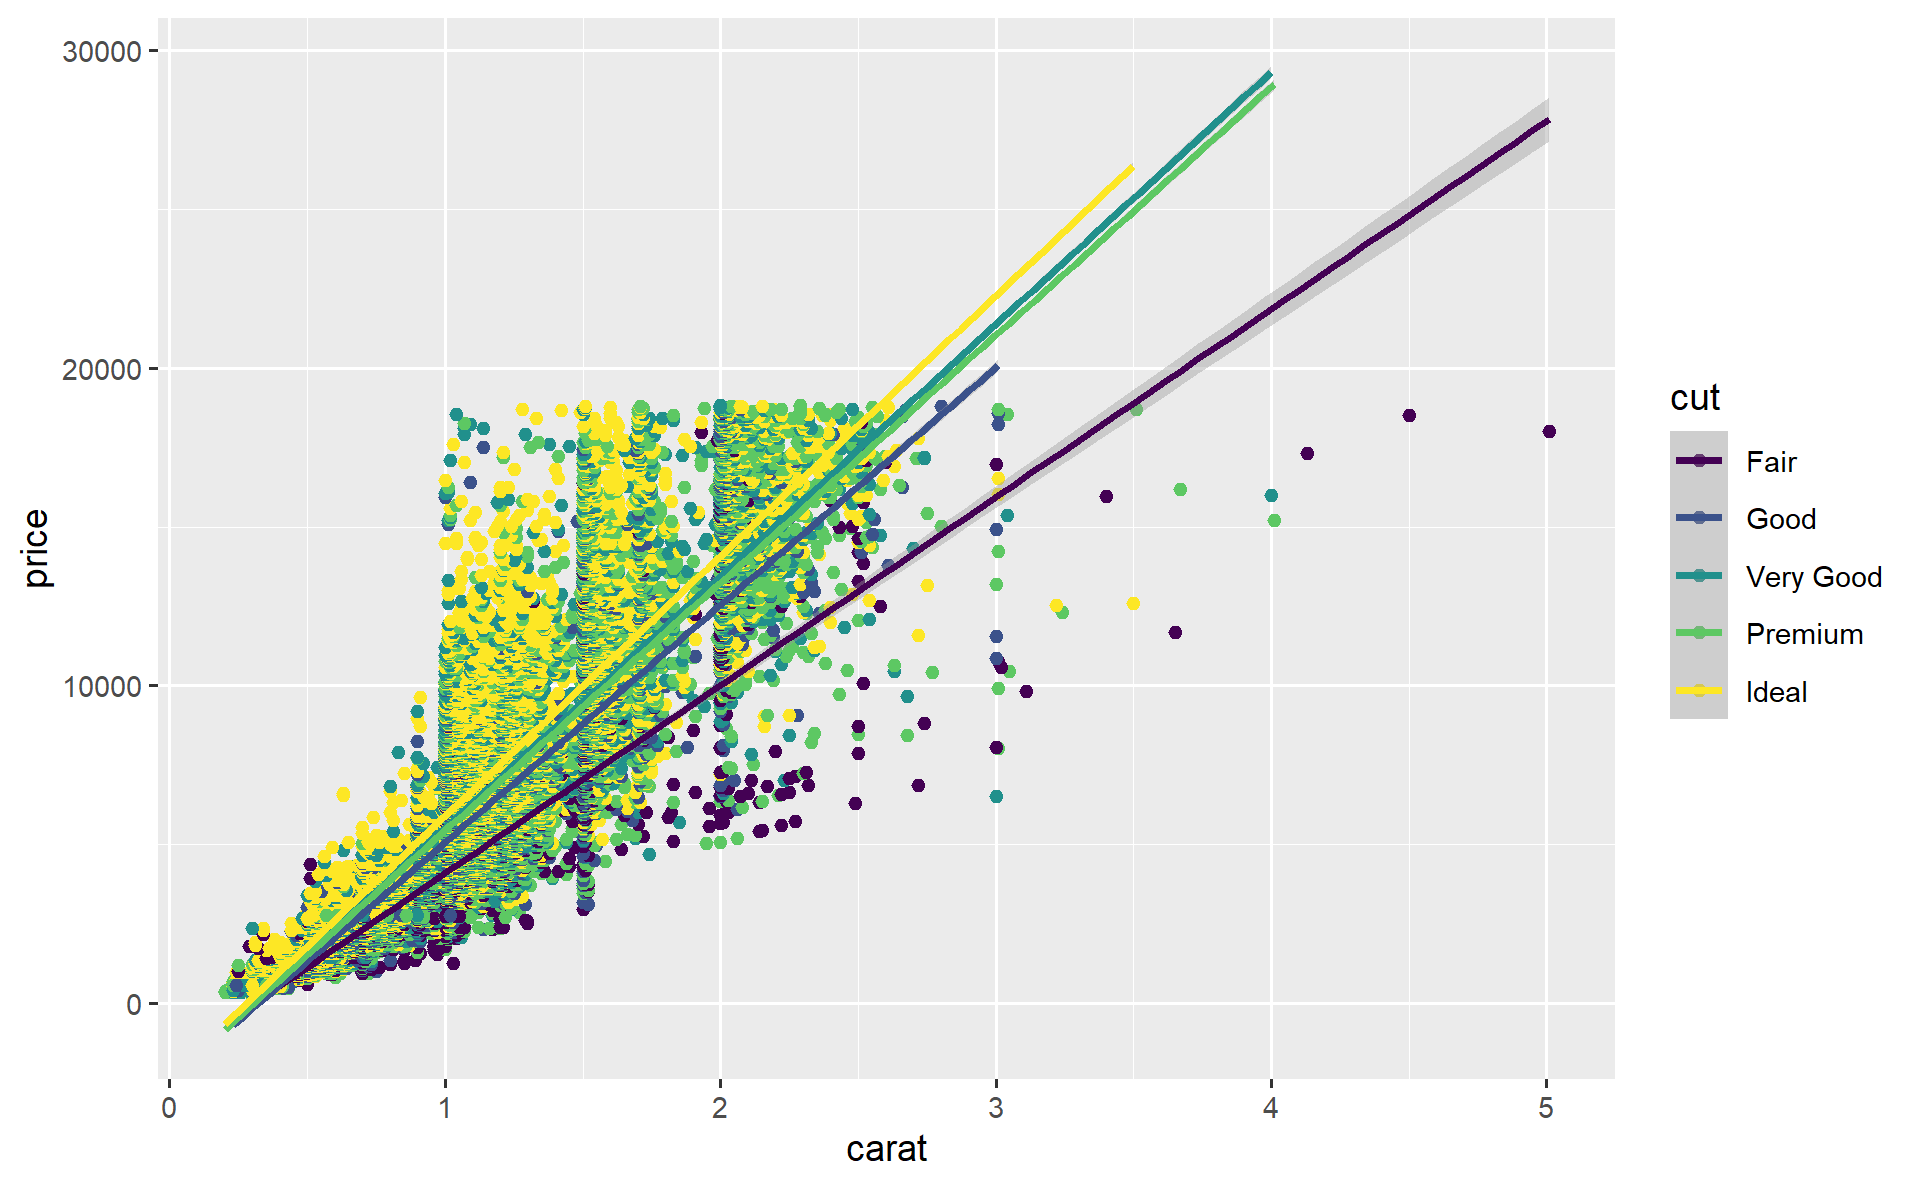
\includegraphics[width=0.7\linewidth]{Data-Analysis-Coursebook_files/figure-latex/unnamed-chunk-27-1} 

}

\caption{Lineáris trend illesztése pontdiagramra}\label{fig:unnamed-chunk-27}
\end{figure}

Mint látjuk jelen esetben a \texttt{geom\_smooth} ugyanazt az \texttt{aes()}-t alkalmazza, mint a \texttt{geom\_point}. Ez azonban problémás, ha nem akarunk a kategorikus ismérv mentén 5 külön trendvonalat illeszteni. Ilyenkor jelent megoldás egy új \texttt{aes()} megadása egyetlen ábrán belül.

\begin{Shaded}
\begin{Highlighting}[]
\FunctionTok{ggplot}\NormalTok{(diamonds) }\SpecialCharTok{+}
  \FunctionTok{geom\_point}\NormalTok{(}\FunctionTok{aes}\NormalTok{(}\AttributeTok{x =}\NormalTok{ carat, }\AttributeTok{y =}\NormalTok{ price, }\AttributeTok{color =}\NormalTok{ cut)) }\SpecialCharTok{+} 
  \FunctionTok{geom\_smooth}\NormalTok{(}\FunctionTok{aes}\NormalTok{(}\AttributeTok{x =}\NormalTok{ carat, }\AttributeTok{y =}\NormalTok{ price), }\AttributeTok{method =} \StringTok{"lm"}\NormalTok{)}
\CommentTok{\#\textgreater{} \textasciigrave{}geom\_smooth()\textasciigrave{} using formula \textquotesingle{}y \textasciitilde{} x\textquotesingle{}}
\end{Highlighting}
\end{Shaded}

\begin{figure}

{\centering 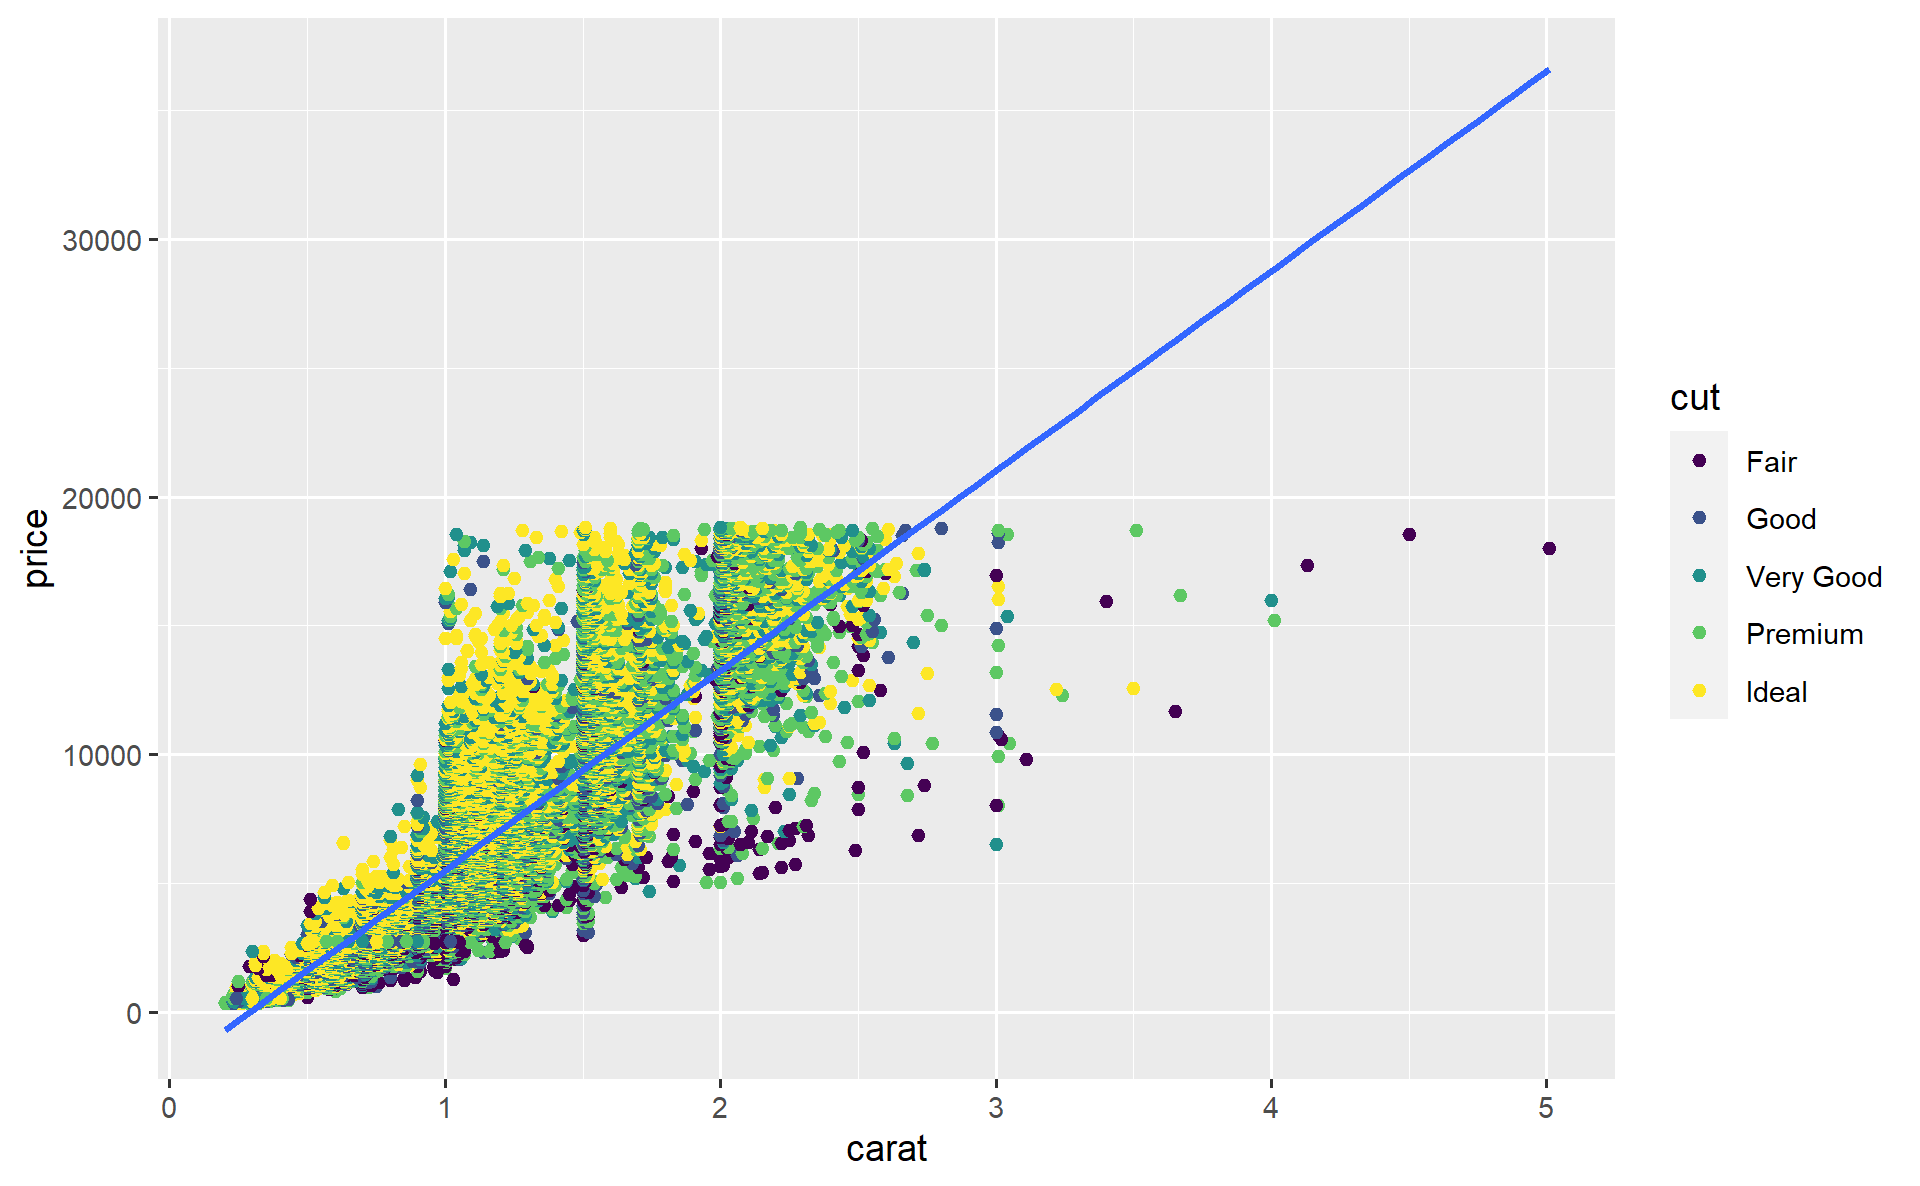
\includegraphics[width=0.7\linewidth]{Data-Analysis-Coursebook_files/figure-latex/unnamed-chunk-28-1} 

}

\caption{Lineáris trend illesztése pontdiagramra két külön esztétika függvénnyel}\label{fig:unnamed-chunk-28}
\end{figure}

\hypertarget{facet}{%
\subsection{Facet}\label{facet}}

A \texttt{facet} az utolsó parancs amit érinteni kívánunk. Ennek segítségével lehetőség van egy ábra felosztására valamely változó mentén. Például a \texttt{cut} változó szerint csoportosítva megtekintve a pontdiagramok:

\begin{Shaded}
\begin{Highlighting}[]
\FunctionTok{ggplot}\NormalTok{(diamonds, }\FunctionTok{aes}\NormalTok{(}\AttributeTok{x =}\NormalTok{ carat, }\AttributeTok{y =}\NormalTok{ price)) }\SpecialCharTok{+}
  \FunctionTok{geom\_point}\NormalTok{() }\SpecialCharTok{+}
  \FunctionTok{facet\_wrap}\NormalTok{(}\SpecialCharTok{\textasciitilde{}}\NormalTok{ cut)}
\end{Highlighting}
\end{Shaded}

\begin{figure}

{\centering 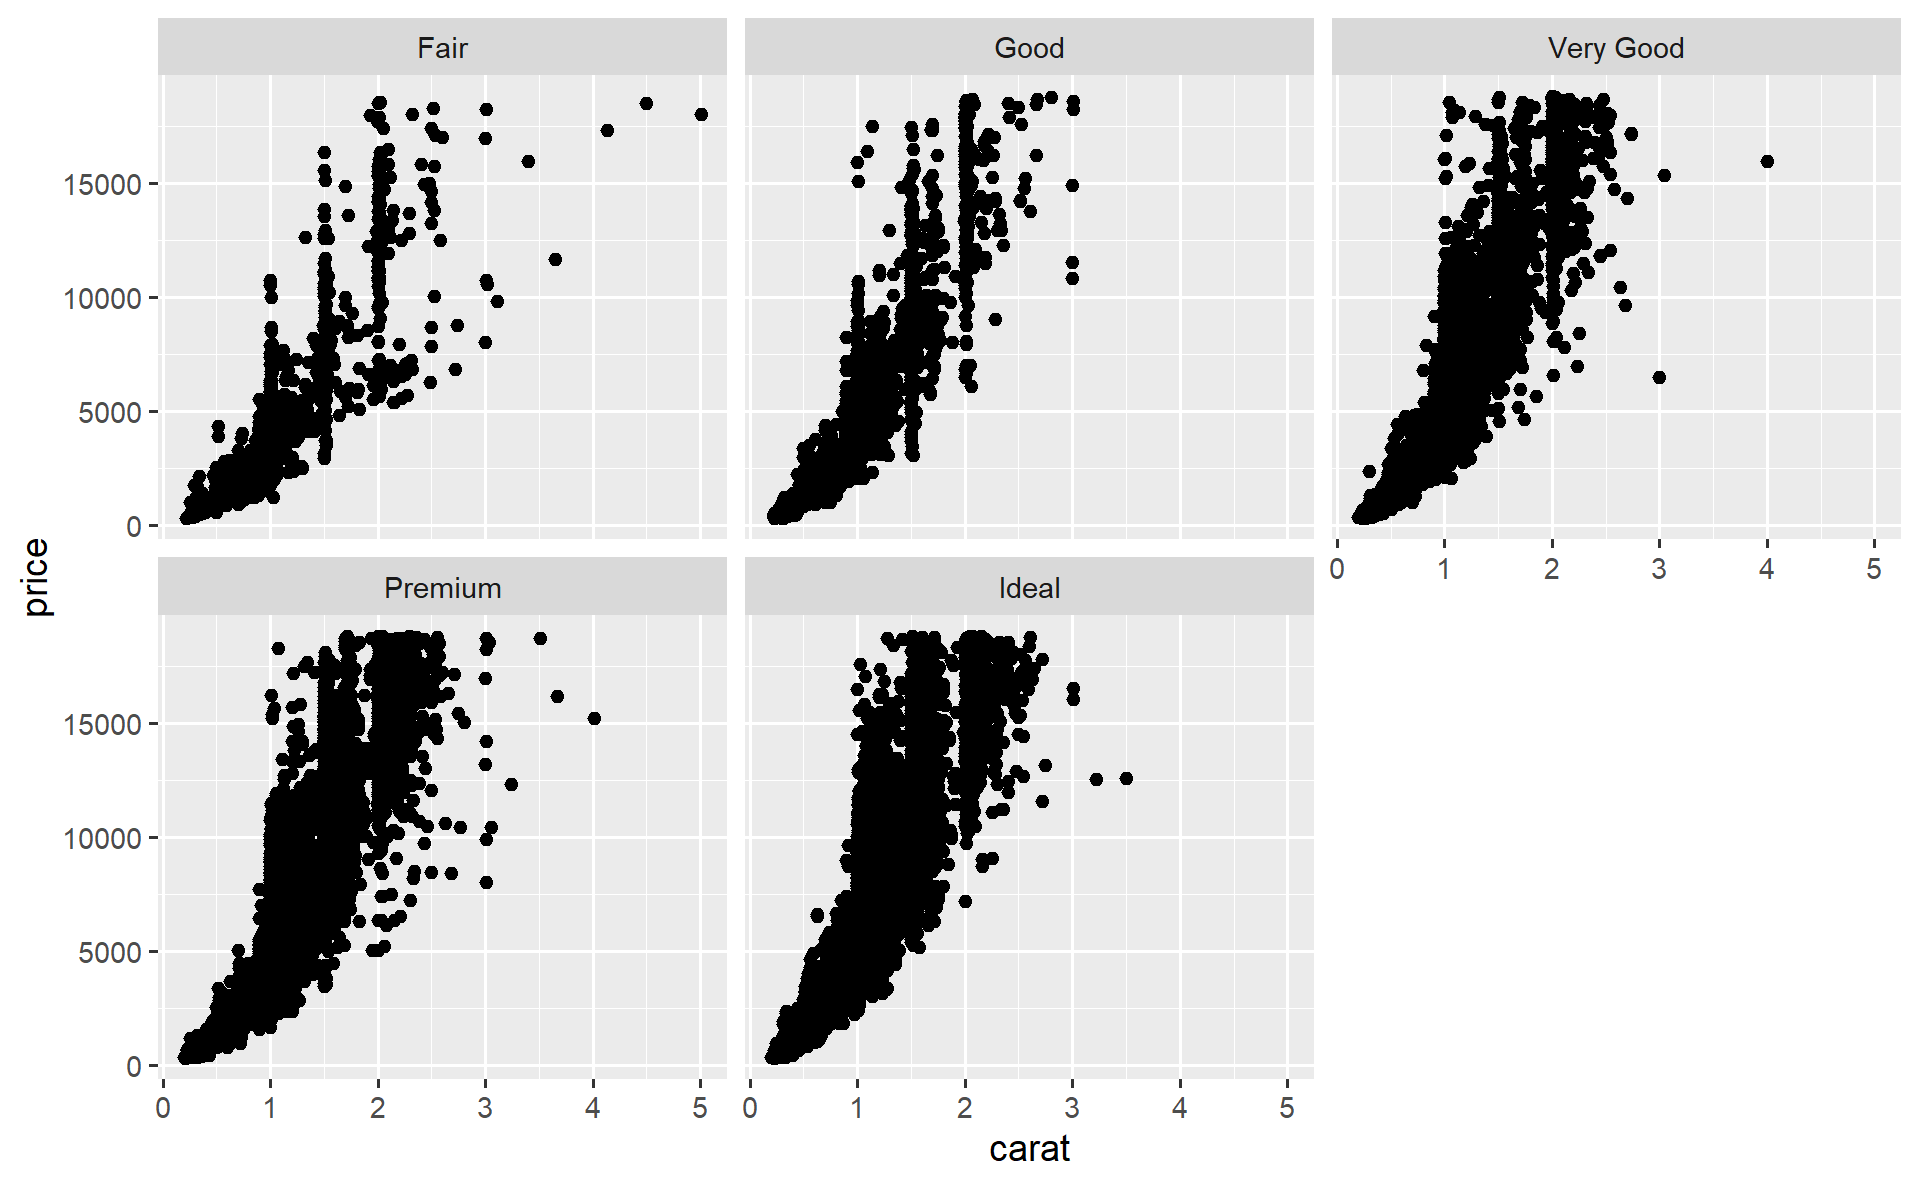
\includegraphics[width=0.7\linewidth]{Data-Analysis-Coursebook_files/figure-latex/unnamed-chunk-29-1} 

}

\caption{Facet alkalmazása egy változó szerint}\label{fig:unnamed-chunk-29}
\end{figure}

Ha pedig soronként és oszloponként is akarunk csoportosítani:

\begin{Shaded}
\begin{Highlighting}[]
\FunctionTok{ggplot}\NormalTok{(diamonds, }\FunctionTok{aes}\NormalTok{(}\AttributeTok{x =}\NormalTok{ carat, }\AttributeTok{y =}\NormalTok{ price)) }\SpecialCharTok{+}
  \FunctionTok{geom\_point}\NormalTok{() }\SpecialCharTok{+}
  \FunctionTok{facet\_grid}\NormalTok{(color }\SpecialCharTok{\textasciitilde{}}\NormalTok{ cut)}
\end{Highlighting}
\end{Shaded}

\begin{figure}

{\centering 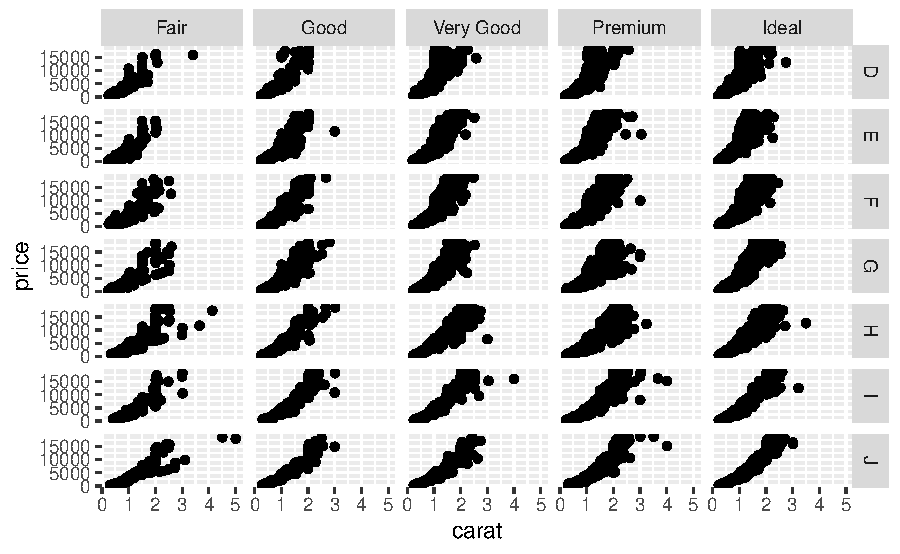
\includegraphics[width=0.7\linewidth]{Data-Analysis-Coursebook_files/figure-latex/unnamed-chunk-30-1} 

}

\caption{Facet alkalmazása két változó szerint}\label{fig:unnamed-chunk-30}
\end{figure}

\hypertarget{kitekintuxe9s}{%
\subsection{Kitekintés}\label{kitekintuxe9s}}

A ggplot2 logikusan felépített működése annyira a felhasználók kedvencévé tette, hogy számos kiegészító package épült rá: \texttt{ggpubs}, \texttt{GGally}, \texttt{gganimate}, stb. Ezek jelenleg nem részei a tananyagnak, azonban érdemes rájuk nézni, ha szakdolgozat vagy TDK prezentálása során szeretnéd lenyűgözni a közönséged. Kedvcsináló:

\hypertarget{part-week-5}{%
\part*{Week 5}\label{part-week-5}}
\addcontentsline{toc}{part}{Week 5}

\hypertarget{lecture5}{%
\section{Lecture 5}\label{lecture5}}

In this chapter, you'll learn how to wrap ggplot2 and dplyr function in a Shiny app.
(If you don't use the tidyverse, you can skip this chapter 😄.) The techniques for wrapping ggplot2 and dplyr functions in a functions and package, are a a little different and covered in other resources like \href{http://ggplot2.tidyverse.org/dev/articles/ggplot2-in-packages.html}{\emph{Using ggplot2 in packages}} or \href{http://dplyr.tidyverse.org/articles/programming.html}{\emph{Programming with dplyr}}.

\hypertarget{tidy-motivation}{%
\subsection{Motivation}\label{tidy-motivation}}

Imagine I want to create an app that allows you to filter a numeric variable to select rows that are greater than a threshold.
You might write something like this:

Let's begin with this call to \texttt{filter()} which uses a data-variable (\texttt{carat}) and an env-variable (\texttt{min}):

\begin{Shaded}
\begin{Highlighting}[]
\FunctionTok{ggplot}\NormalTok{(cars, }\FunctionTok{aes}\NormalTok{(speed, dist)) }\SpecialCharTok{+} 
  \FunctionTok{geom\_point}\NormalTok{()}
\end{Highlighting}
\end{Shaded}

\begin{center}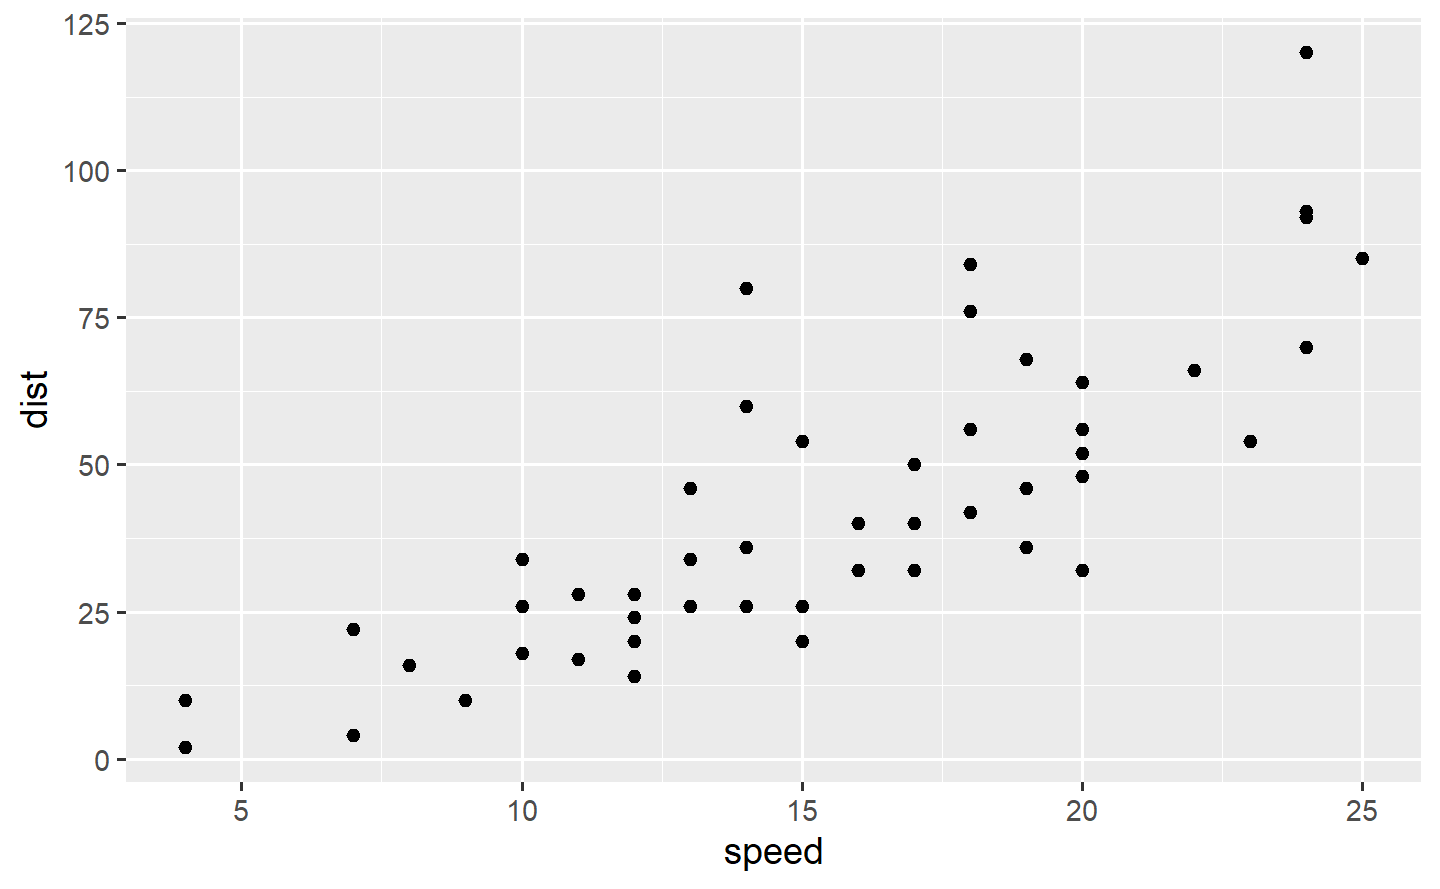
\includegraphics[width=0.7\linewidth]{Data-Analysis-Coursebook_files/figure-latex/unnamed-chunk-32-1} \end{center}

\hypertarget{seminar5}{%
\section{Seminar 5}\label{seminar5}}

\hypertarget{part-week-6}{%
\part*{Week 6}\label{part-week-6}}
\addcontentsline{toc}{part}{Week 6}

\hypertarget{lecture6}{%
\section{Lecture 6}\label{lecture6}}

In this chapter, you'll learn how to wrap ggplot2 and dplyr function in a Shiny app.
(If you don't use the tidyverse, you can skip this chapter 😄.) The techniques for wrapping ggplot2 and dplyr functions in a functions and package, are a a little different and covered in other resources like \href{http://ggplot2.tidyverse.org/dev/articles/ggplot2-in-packages.html}{\emph{Using ggplot2 in packages}} or \href{http://dplyr.tidyverse.org/articles/programming.html}{\emph{Programming with dplyr}}.

\hypertarget{tidy-motivation}{%
\subsection{Motivation}\label{tidy-motivation}}

Imagine I want to create an app that allows you to filter a numeric variable to select rows that are greater than a threshold.
You might write something like this:

Let's begin with this call to \texttt{filter()} which uses a data-variable (\texttt{carat}) and an env-variable (\texttt{min}):

\begin{Shaded}
\begin{Highlighting}[]
\FunctionTok{ggplot}\NormalTok{(cars, }\FunctionTok{aes}\NormalTok{(speed, dist)) }\SpecialCharTok{+} 
  \FunctionTok{geom\_point}\NormalTok{()}
\end{Highlighting}
\end{Shaded}

\begin{center}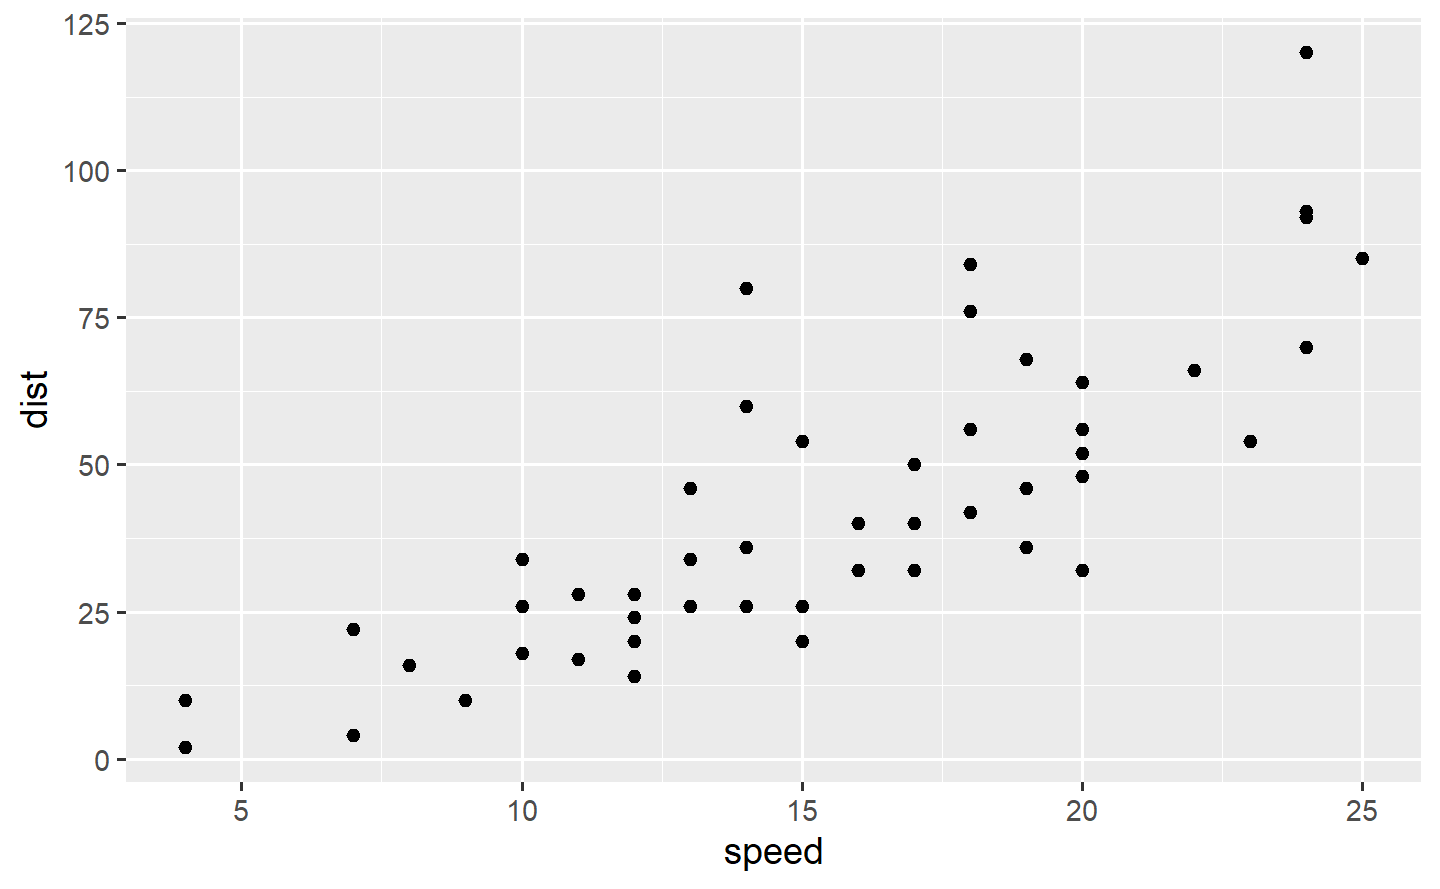
\includegraphics[width=0.7\linewidth]{Data-Analysis-Coursebook_files/figure-latex/unnamed-chunk-33-1} \end{center}

\hypertarget{seminar6}{%
\section{Seminar 6}\label{seminar6}}

In this chapter, you'll learn how to wrap ggplot2 and dplyr function in a Shiny app.
(If you don't use the tidyverse, you can skip this chapter 😄.) The techniques for wrapping ggplot2 and dplyr functions in a functions and package, are a a little different and covered in other resources like \href{http://ggplot2.tidyverse.org/dev/articles/ggplot2-in-packages.html}{\emph{Using ggplot2 in packages}} or \href{http://dplyr.tidyverse.org/articles/programming.html}{\emph{Programming with dplyr}}.

\hypertarget{tidy-motivation}{%
\subsection{Motivation}\label{tidy-motivation}}

Imagine I want to create an app that allows you to filter a numeric variable to select rows that are greater than a threshold.
You might write something like this:

Let's begin with this call to \texttt{filter()} which uses a data-variable (\texttt{carat}) and an env-variable (\texttt{min}):

\begin{Shaded}
\begin{Highlighting}[]
\FunctionTok{ggplot}\NormalTok{(cars, }\FunctionTok{aes}\NormalTok{(speed, dist)) }\SpecialCharTok{+} 
  \FunctionTok{geom\_point}\NormalTok{()}
\end{Highlighting}
\end{Shaded}

\begin{center}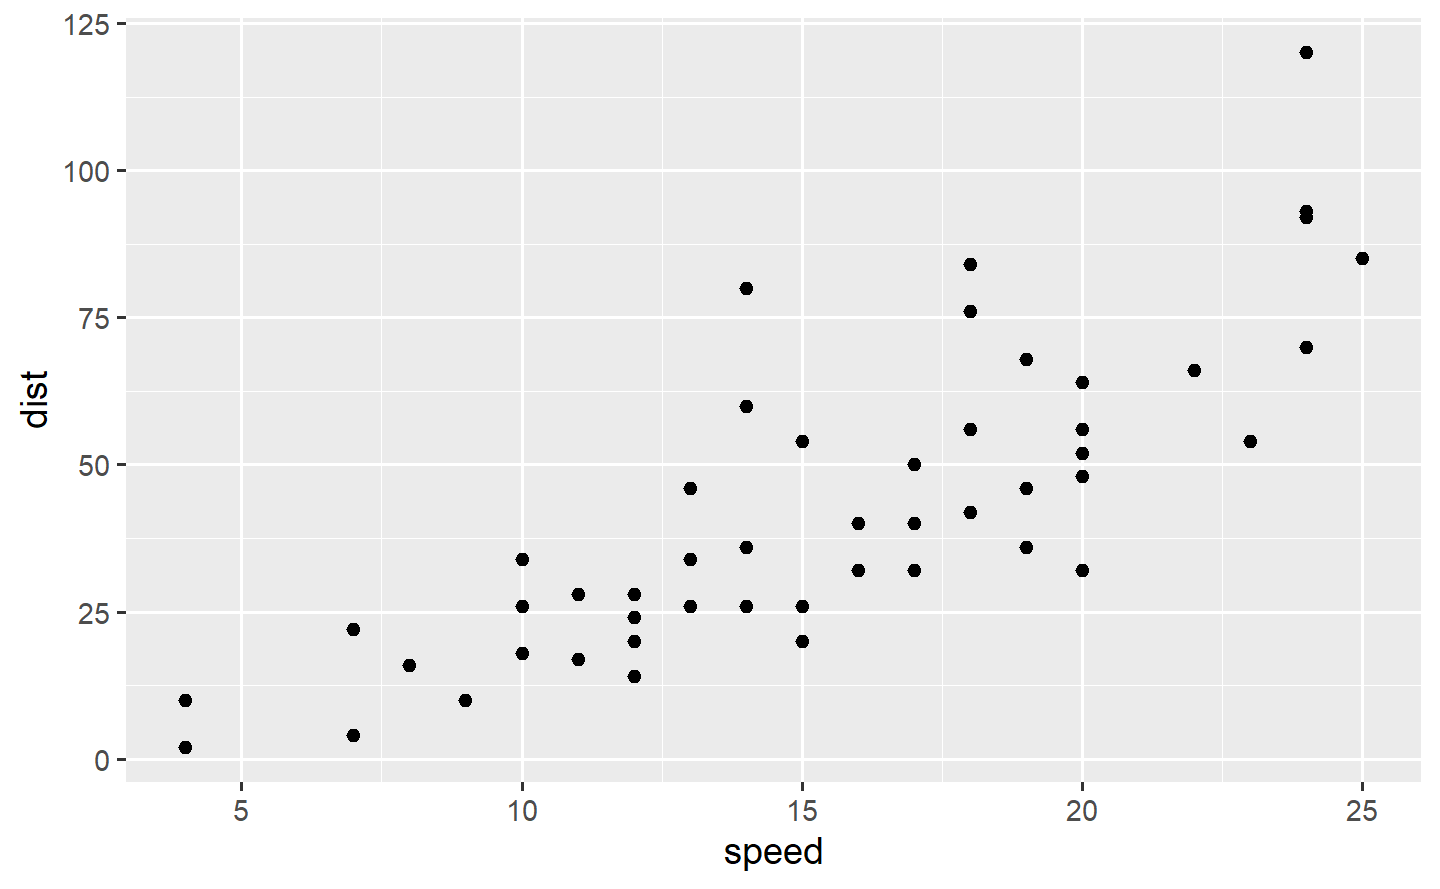
\includegraphics[width=0.7\linewidth]{Data-Analysis-Coursebook_files/figure-latex/unnamed-chunk-34-1} \end{center}

\hypertarget{part-week-7}{%
\part*{Week 7}\label{part-week-7}}
\addcontentsline{toc}{part}{Week 7}

\hypertarget{lecture7}{%
\section{Lecture 7}\label{lecture7}}

In this chapter, you'll learn how to wrap ggplot2 and dplyr function in a Shiny app.
(If you don't use the tidyverse, you can skip this chapter 😄.) The techniques for wrapping ggplot2 and dplyr functions in a functions and package, are a a little different and covered in other resources like \href{http://ggplot2.tidyverse.org/dev/articles/ggplot2-in-packages.html}{\emph{Using ggplot2 in packages}} or \href{http://dplyr.tidyverse.org/articles/programming.html}{\emph{Programming with dplyr}}.

\hypertarget{tidy-motivation}{%
\subsection{Motivation}\label{tidy-motivation}}

Imagine I want to create an app that allows you to filter a numeric variable to select rows that are greater than a threshold.
You might write something like this:

Let's begin with this call to \texttt{filter()} which uses a data-variable (\texttt{carat}) and an env-variable (\texttt{min}):

\begin{Shaded}
\begin{Highlighting}[]
\FunctionTok{ggplot}\NormalTok{(cars, }\FunctionTok{aes}\NormalTok{(speed, dist)) }\SpecialCharTok{+} 
  \FunctionTok{geom\_point}\NormalTok{()}
\end{Highlighting}
\end{Shaded}

\begin{center}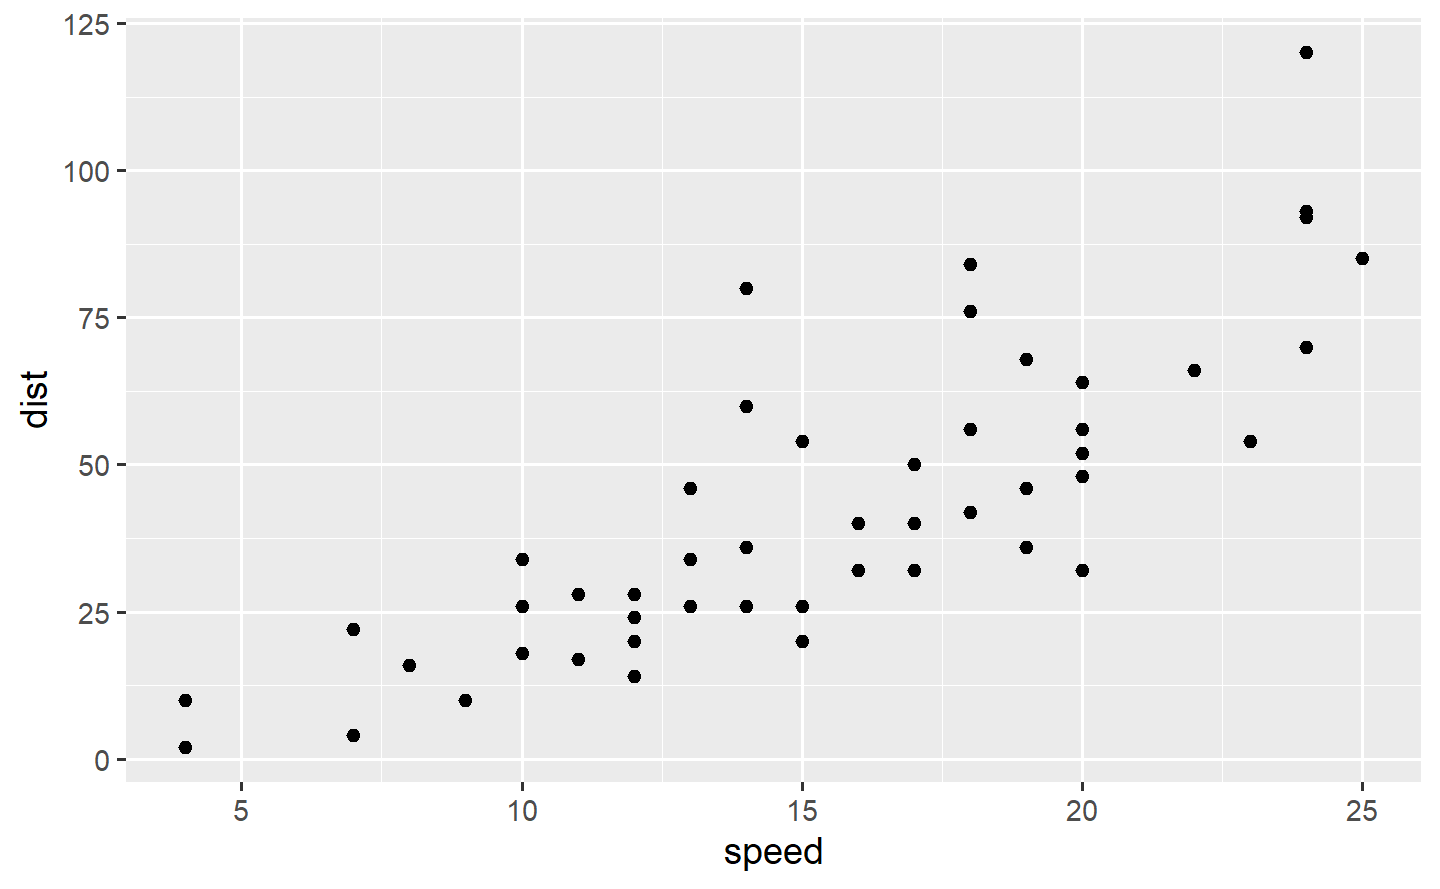
\includegraphics[width=0.7\linewidth]{Data-Analysis-Coursebook_files/figure-latex/unnamed-chunk-35-1} \end{center}

\hypertarget{seminar7}{%
\section{Seminar 7}\label{seminar7}}

In this chapter, you'll learn how to wrap ggplot2 and dplyr function in a Shiny app.
(If you don't use the tidyverse, you can skip this chapter 😄.) The techniques for wrapping ggplot2 and dplyr functions in a functions and package, are a a little different and covered in other resources like \href{http://ggplot2.tidyverse.org/dev/articles/ggplot2-in-packages.html}{\emph{Using ggplot2 in packages}} or \href{http://dplyr.tidyverse.org/articles/programming.html}{\emph{Programming with dplyr}}.

\hypertarget{tidy-motivation}{%
\subsection{Motivation}\label{tidy-motivation}}

Imagine I want to create an app that allows you to filter a numeric variable to select rows that are greater than a threshold.
You might write something like this:

Let's begin with this call to \texttt{filter()} which uses a data-variable (\texttt{carat}) and an env-variable (\texttt{min}):

\begin{Shaded}
\begin{Highlighting}[]
\FunctionTok{ggplot}\NormalTok{(cars, }\FunctionTok{aes}\NormalTok{(speed, dist)) }\SpecialCharTok{+} 
  \FunctionTok{geom\_point}\NormalTok{()}
\end{Highlighting}
\end{Shaded}

\begin{center}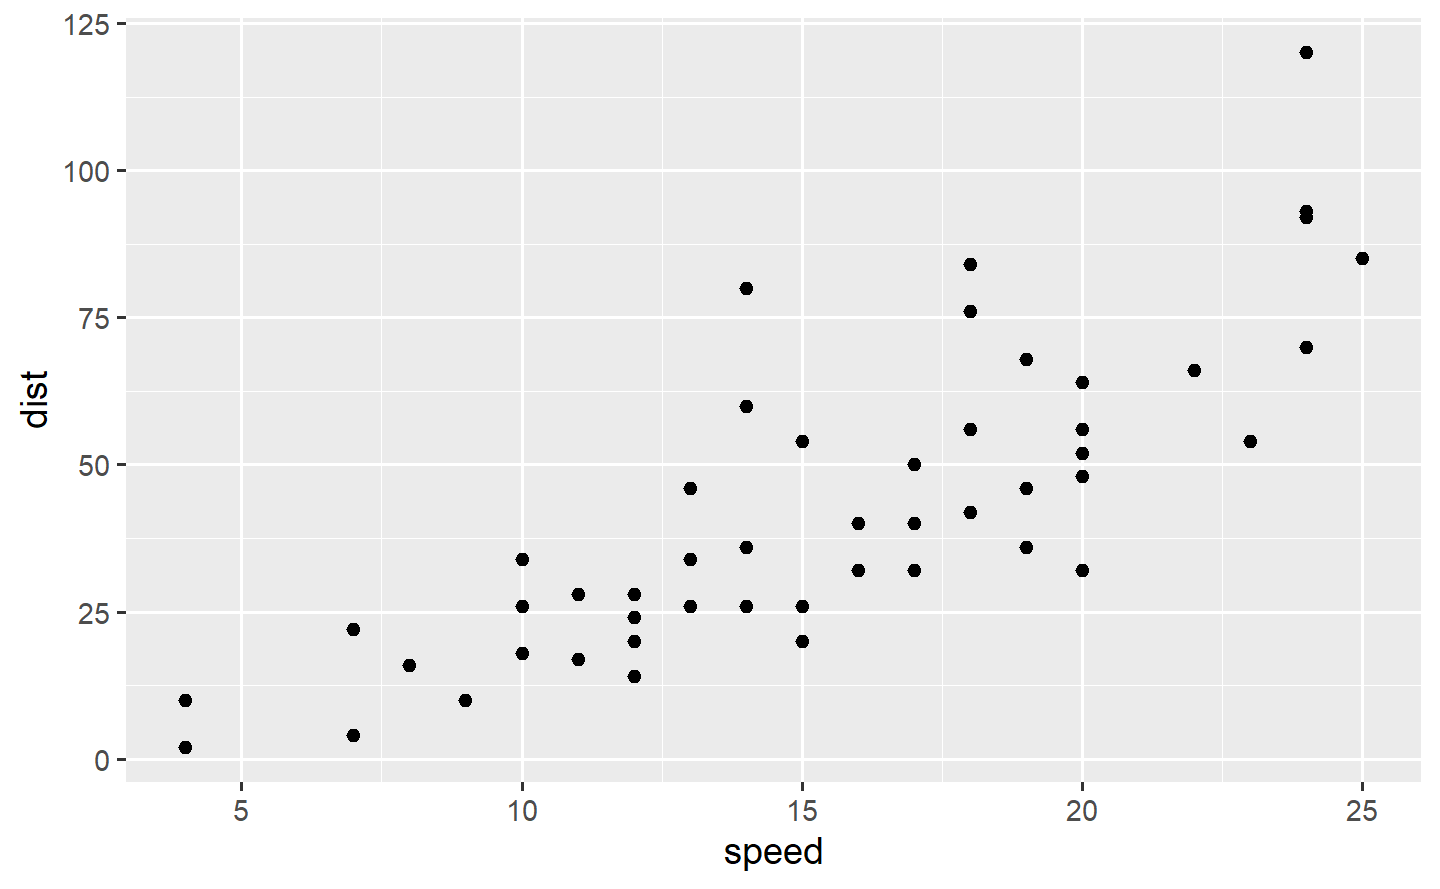
\includegraphics[width=0.7\linewidth]{Data-Analysis-Coursebook_files/figure-latex/unnamed-chunk-36-1} \end{center}

  \bibliography{references.bib}

\end{document}
